%%
%% Arquivo principal da tese ou dissertação.
%%
%% Siga as instruções que seguem comentadas neste arquivo.
%%
%% ESTA VERSÃO REQUER UM EDITOR UTF-8.
%%
%% Exemplos de utilização dos comandos podem ser encontrados
%% nos capítulos que acompanham este pacote.
%%
%%
\documentclass[mestrado,codelist]{ppgeq}
%\documentclass[doutorado]{ppgeq}
%\documentclass[qualify]{ppgeq}

% algumas customizações: o preamble.tex pode ser editado pelo usuário
%%+++++++++++++++++++++++++++++++++++++++ Preâmbulo ++++++++++++++++++++++++++++++++++++++++++++++++++++++++++++++++
%%   Preâmbulo: pacotes, configurações e comandos específicos do usuário

%+++++++++++++++++++++++++++++++++++++++ Pacotes de Macros ++++++++++++++++++++++++++++++++++++++++++++++++++++++++++++++++
\usepackage{color} 		% Pacote para cores
\usepackage{graphicx} 	% Pacote para graficos
\usepackage{url}		% Pacote para inserir URL
\usepackage{extarrows} 	% Pacote para inserir formulas quimicas
\usepackage{framed} 	% Pacote para inserir frames em textos e figuras
\usepackage[version=3]{mhchem} % Formulas químicas automaticas, comando \ce{}

%+++++++++++++++++++++++++++++++++++++++ Definições do listings ++++++++++++++++++++++++++++++++++++++++++++++++++++++++++++++++
% Sintaxe do EMSO
\lstdefinelanguage{EMSO}{
  morekeywords={
		Model,FlowSheet,Estimation,Optimization,
		PARAMETERS,VARIABLES,EQUATIONS,DEVICES,SET,SPECIFY,GUESS,CONNECTIONS,
		INITIAL,OPTIONS,ATTRIBUTES,ESTIMATE,EXPERIMENTS,MINIMIZE,MAXIMIZE,FREE,
		Brief,Unit,DisplayUnit,Default,Upper,Lower,Type,final,Valid,Symbol,PosX,PosY,
		Components,LiquidModel,VapourModel,
		Pallete,Icon,Info,Protected,Hidden,
		TimeStep,TimeEnd,TimeUnit,Dynamic,SparseAlgebra,NLPSolver,NLPSolveNLA,NLASolver,DAESolver,
		File,RelativeAccuracy,AbsoluteAccuracy,EventAccuracy,MaxIterations,GuessFile,InitialFile,
		Statistics,Fit,Parameter,Prediction,Significance,BiLateral,RunTests,NumJac,
		using,for,as,to,if,end,else,switch,switchto,when,case,
		in,out,outer, 
		Integer,Real,Boolean,Text,Plugin,Switcher,CalcObject,
		equal,and,or,true,false,
        time,diff,sum,sumt,prod,prodt,transp,min,max,abs,
		sign,round,sinh,cosh,tanh,coth,atan,
		exp,log,ln,sqrt,sin,cos,tan,asin,acos},
  sensitive = true,
  morecomment=[l]{\#},
  morecomment=[s]{\#*}{*\#},
  morestring=[b]",
  morestring=[b]'
}
\lstset{
  basicstyle=\fontfamily{pcr}\fontseries{m}\selectfont\footnotesize,
  commentstyle=\color[rgb]{0,0.5,0}\itshape,
  keywordstyle=\color{blue}\bfseries,
  stringstyle=\color[rgb]{0.5,0,0.5}\itshape,
  showstringspaces=false,
  numbers=left,
  numberstyle=\fontfamily{pcr}\fontseries{m}\selectfont\tiny,
  numberblanklines=false,
  showlines=false,
  belowskip=\bigskipamount{},
  breaklines=true,
  %stepnumber=2,
  tabsize=6,
  %extendedchars=true,
  %float=h,
  frame=tb
}
%+++++++++++++++++++++++++++++++++++++++ Definições em Comandos ++++++++++++++++++++++++++++++++++++++++++++++++++++++++++++++++
\newcommand{\code}[1]{\texttt{#1}}
\renewcommand{\lstlistingname}{Código}
\renewcommand{\lstlistlistingname}{Lista de Códigos}
\newcommand{\email}{\begingroup \urlstyle{rm}\Url}
\newcommand{\lattes}[2]{\htmladdnormallink{#1}{http://lattes.cnpq.br/#2}} % Curriculo Lattes
%EXEMPLO:
%\lattes{Prof. Dr. José Goldemberg}{1388529283382853}
%onde o link fica http://lattes.cnpq.br/1388529283382853
%estas URLs curtas estão loga após o resumo dos currículos Lattes

%\newcommand{\emso}{{\scshape\fontfamily{cmss}emso}}
\newcommand{\vrtherm}{VRTherm}
\newcommand{\emso}{EMSO}
\newcommand{\emsoname}{\textbf{E}nvironment for \textbf{M}odeling,
	\textbf{S}imulation and \textbf{O}ptimization}
\newcommand{\eml}{EML}
\newcommand{\emlname}{\emso{} \textbf{M}odel \textbf{L}ibrary}
\newcommand{\flowsheet}{\code{FlowSheet}}
\newcommand{\device}{\code{Device}}
\newcommand{\model}{\code{Model}}
\newcommand{\script}{\code{Script}}
\newcommand{\mso}{\code{.mso}}
% The types
\newcommand{\real}{\code{Real}}
\newcommand{\integer}{\code{Integer}}
%\newcommand{\boolean}{\code{Boolean}}
\newcommand{\calcObject}{\code{CalcObject}}
\newcommand{\brief}{\code{Brief}}
\newcommand{\lowerb}{\code{Lower}}
\newcommand{\upperb}{\code{Upper}}

\newcounter{numero}
% Renew the lists to remove the space before it
\renewenvironment{itemize}{\vspace{-\parskip}\vspace{\lineskip}\begin{list}{$\bullet$}
{\usecounter{numero} \setlength{\rightmargin}{\leftmargin}}}{\end{list}}
\renewenvironment{enumerate}{\vspace{-\parskip}\vspace{\lineskip}\begin{list}{\arabic{numero}.}
{\usecounter{numero} \setlength{\rightmargin}{\leftmargin}}}{\end{list}}

%List in roman i), ii), etc
\newenvironment{rlist}{\begin{list}{\roman{numero})}
{\usecounter{numero} \setlength{\rightmargin}{\leftmargin}}}{\end{list}}

%List in ROMAN I., II., etc
\newenvironment{Rlist}{\begin{list}{\Roman{numero}.}
{\usecounter{numero} \setlength{\rightmargin}{\leftmargin}}}{\end{list}}

%List in alph a), b), etc
\newenvironment{alist}{\begin{list}{\alph{numero})}
{\usecounter{numero} \setlength{\rightmargin}{\leftmargin}}}{\end{list}}

%List in Alph A), B), etc
\newenvironment{Alist}{\begin{list}{\Alph{numero})}
{\usecounter{numero} \setlength{\rightmargin}{\leftmargin}}}{\end{list}}

%List in arabic 1), 2), etc
\newenvironment{nlist}{\begin{list}{\arabic{numero})}
{\usecounter{numero} \setlength{\rightmargin}{\leftmargin}}}{\end{list}}

%\nomenclature[G]{$\alpha$}{Constant}
%\nomenclature[A]{$x$}{Variable}
%\nomenclature{$l$}{Length\nomunit{$m$}}

%+++++++++++++++++++++++++++++++++++++++ Desta linha para baixo não modifique ++++++++++++++++++++++++++++++++++++++++++++++++++



% modifique os argumentos dos comandos abaixo para que as primeiras páginas
% sejam construídas automaticamente
\title{Padrão de Dissertação/Tese/Qualify do PPGEQ--UFRGS}
\author{Fulano de Tal}
\authorCitation{Tal, Fulano de}
\area{Pesquisa e Desenvolvimento de Processos}
\tyear{2014}
% verificar o número de páginas do PDF final
\totalPages{146}
\advisor{Rafael de Pelegrini Soares}
\advisorCitation{Soares, Rafael de P.}
\coadvisor{Beltrano de Tal} % opcional
\coadvisorCitation{Tal, Beltrano de}
% \coadvisorCitation{Tal, Beltrano de}
\bancai{Prof. Banca 1, D.Sc.}
\bancaii{Prof. Banca 2, Ph.D.}
\bancaiii{Prof. Banca 3, D.Sc}
% \bancaiiii{Prof. Banca 4, D.Sc} % opcional
\pensamento{pensamento.\\ \vspace{0.5cm} \begin{flushright}
Autor \end{flushright}}
\agradecimento{Agradecimentos....
}

\resumo{A pesquisa acerca da modelagem de colunas de destilação não é mais uma
novidade nos dias de hoje. Os primeiros trabalhos, com metodologias propostas para a 
solução de sistemas de separação modelados prato a prato, surgiram na década de 30. Porém,
só a partir da década de 50, com o advento do computador digital, foram realizados 
investimentos sólidos no desenvolvimento de novos algoritmos e simuladores. Apesar 
deste investimento, apenas modelos simplificados eram utilizados devido 
à baixa capacidade de processamento. A partir da década de 70, os primeiros simuladores 
comerciais começaram a ser introduzidos na indústria e o desenvolvimento de modelos rigorosos 
não parou mais.
Dentro deste contexto, este trabalho tem como objetivo o desenvolvimento de um modelo 
rigoroso de coluna de destilação, genérico, dinâmico e de fácil aplicação nos mais variados
tipos de estudos, desde simples simulações de operação até otimizações e previsões de comportamentos
de parada e partida de plantas. Ou seja, um modelo projetado para situações onde uma representação fiel
do comportamento dinâmico é necessária. Os modelos gerados neste estudo foram implementados na linguagem
de modelagem do simulador \emso\ e fazem parte da biblioteca EML (EMSO Model Library). Esta biblioteca
é distribuída no conceito de \emph{software} livre, disponibilizando todos os
modelos via internet e sem custo.
Para a validação dos modelos desenvolvidos foram utilizados dois exemplos: uma
coluna de destilação reativa com dados provenientes da literatura e uma coluna
deisobutanizadora industrial da PETROBRAS com 80 pratos que separa o isobutano de uma
mistura de 13 componentes.
Este último problema resulta em um sistema com mais de 6300 variáveis,
provando que o simulador utilizado é muito eficiente para a resolução de
problemas de grande escala. Os resultados da validação foram
satisfatórios, assim como o desempenho do simulador \emso\ quanto à eficiência
computacional e à robustez na solução do problema. }
\palavraschave{1.~Destilação. 2.~Modelagem. 3.~Simulação Dinâmica. 4.~Colunas de pratos.}

\abstract{At present, at least for engineering purposes, the most successful
predictive models for activity coefficients are those based on functional
groups, such as UNIFAC and its variants. While these models require large
amounts of experimental data, the ones based on COSMO-RS require the calibration
of a small set of universal parameters. However, the resolution required by
engineering tasks, such as the optimization of separation systems, is higher
than that obtained by COSMO-RS models. Thus, in this work a novel
Functional-Segment Activity Coefficient (F-SAC) model is proposed. This new
model is also based on the concept of functional groups, but the interaction
energy between groups comes from the COSMO-RS theory.
% The proposed model considers
% that each pure substance consists of several neutral functional groups (with
% global charge zero) and the model parameters are the apparent surface charges of
% each group.
In this study, we considered only mixtures where there is no formation of
hydrogen bonds or when they could be assumed negligible. Then, only three
parameters were required to describe each functional group. In principle, once
the parameters for each functional group are properly calibrated, they should
work to describe the interactions with any other group. This is the main
advantage of the proposed model, the number of model parameters grows linearly
with the number of functional groups, whereas in UNIFAC the number of
interaction parameters exhibit quadratic growth with respect to the number of
groups. For the experimental database of infinite dilution activity coefficients
considered, the correlation of F-SAC have shown a mean absolute error of 0.07
ln-unit. The UNIFAC~(Do) and COSMO-SAC models presented errors of 0.12 and 0.21,
respectively. F-SAC was also evaluated for more than 1000 binary mixtures
of solute in ionic liquid with data available in the literature.
Again, the model have shown good correlation to the experimental data,
with mean absolute error of 0.17
ln-unit, similar to the performance with the organic mixtures. The predictive strength
of the model was assessed by using vapor-liquid equilibrium data not
considered in the model fitting process. Very good agreement with experimental
data was possible over the entire composition range, as well as in the
prediction of azeotropes.
These results demonstrate the potential of the proposed method. }
\keywords{1.Activity Coefficient. 2.COSMO. 3.UNIFAC. 4.IDAC. 5.VLE. 6.Ionic Liquid.}

% Desse ponto modifique apenas a inclusão dos capítulos e apêndices
\begin{document}

% hifenizacao
% hifenizacao
\hyphenation{
a-ce-le-ra-\c{c}\~ao
a-com-pa-nha-do a-com-pa-nhar
a-de-qua-da
a-di-ci-o-na-das
a-li-men-ta-\c{c}\~ao
al-te-ra-das
a-que-ci-men-to
a-na-li-sa-dos
a-pre-sen-ta a-pre-sen-ta-do a-pre-sen-ta-da a-pre-sen-tam a-pre-sen-ta-ram a-pre-sen-ta-dos
ba-lan-ços
bo-lhas bo-lha
ca-mi-nho
ca-rac-te-ri-za-\c{c}\~ao
ca-rac-te-ri-zam
ca-te-go-ri-as
cha-ma-do
co-lo-ri-do
co-lu-nas co-lu-na
co-mer-ci-ais
con-si-de-ra-\c{c}\~ao con-si-de-ra-\c{c}\~oes con-si-de-ra-do con-si-de-ra-das
con-si-de-ra-da con-si-de-ra-das
con-si-de-r\'a-veis
co-nhe-ci-do
cor-res-pon-dem
de-cla-ran-do de-cla-rar
de-com-po-si-\c{c}\~ao
des-co-bri-ram
des-co-lo-ri-dos
des-con-ti-nu-i-da-de
de-ta-lhes
de-ter-mi-ne
di-fe-ren-te di-fe-ren-ci-ais
di-fe-ren-ci-a-\c{c}\~ao
di-fe-ren-\c{c}a
di-fe-ren-ci-ar
dif-fer-en-tial
di-n\^a-mi-co
di-re-ci-o-na-das
dis-po-n\'i-vel dis-po-n\'i-veis
do-cu-men-to
e-mu-lar
e-ner-gi-a
e-qua-\c{c}\~oes
e-qui-pa-men-to
e-qui-vo-ca-da
es-pe-ra-do
es-ta-be-le-ci-dos
es-ta-bi-li-da-de
es-tra-t\'e-gi-ca
e-xa-ta-men-te
e-xem-plo e-xem-pli-fi-ca-do
ex-pe-ri-men-to
i-ni-ci-a-li-za-\c{c}\~ao
fi-gu-ras fi-gu-ra
for-ma-li-za-\c{c}\~ao
for-ne-ci-do
ga-nhan-do
ge-ra-do
hi-dro-di-n\^a-mi-ca
hi-dro-di-n\^a-mi-co
lo-ca-li-za-\c{c}\~ao
li-mi-ta-\c{c}\~oes
l\'i-qui-do
li-te-ra-tu-ra
Men-del-sohn
me-no-res
mo-di-fi-ca-\c{c}\~ao
mo-di-fi-ca-da
mo-de-lo mo-de-los mo-de-la-gem
na-tu-ral-men-te
ne-ces-s\'a-ri-a ne-ces-s\'a-ri-as
nu-m\'e-ri-co
nu-m\'e-ri-ca
o-pe-ra-\c{c}\~ao
or-to-go-nal
or-to-go-nais
ou-tros ou-tras
pa-r\^a-me-tros pa-r\^a-me-tro
par-ti-cu-la-res
pes-qui-sa-do-res
po-si-ti-vos po-si-ti-vo
pri-mei-ra
pro-ble-ma pro-ble-mas
pro-cu-ra
quan-do
re-a-li-da-de
re-a-li-za-das
re-a-li-za-da
re-es-cre-ven-do
re-flu-xa-do
res-pei-to
res-pos-ta
res-tri-\c{c}\~oes
re-fe-r\^en-cias
re-le-van-tes
re-pre-sen-ta-do
ri-go-ro-so ri-go-ro-sos ri-go-ris-mo
sa-tu-ra-da sa-tu-ra-do
se-me-lhan-\c{c}a se-me-lhan-\c{c}as
se-pa-ran-do
so-lu-\c{c}\~ao
si-mu-la-dor
si-mu-la-tor
si-mu-la-\c{c}\~oes si-mu-la-\c{c}\~ao
si-mul-ta-nea-men-te
subs-ti-tu-i-\c{c}\~ao
tem-pe-ra-tu-ra tem-pe-ra-tu-ras
ter-mo-di-n\^a-mi-co
trans-fe-rên-cia
u-ti-li-zam
va-po-ri-za-da
va-ri-\'a-veis
vi-su-a-li-za-do
}

\maketitle

% Inclusao dos Capítulos
%
% 
%
\chapter{Introdução} \label{chap:introduction}

\emph{Isto é uma sinopse de capítulo. A ABNT não traz nenhuma normatização a
respeito desse tipo de resumo, que é mais comum em romances e livros técnicos.
}


A operação de separação de componentes de uma mistura por destilação tem uma longa história. Credita-se a sua
descoberta aos chineses durante a dinastia de Chou (221 a 1122 d.C.). Desde então, a produção de bebidas destiladas,
as chamadas ``bebidas dos deuses'', evoluíram juntamente com o progresso da civilização. Primeiro na Índia, depois na
Arábia e posteriormente na Inglaterra, em torno de 500 d.C., com a produção de ``mead'', uma bebida alcóolica
resultante da fermentação de mel e água. Mas surpreendentemente, apenas um milênio depois, por volta de 1500 d.C.,
tem-se notícia do primeiro uísque destilado na Escócia \apud{Forbes:1948}{Lockett:1986}. Embora a produção de bebidas
alcóolicas tenha uma grande importância no descobrimento e desenvolvimento da operação de destilação, nos dias de hoje,
a sua utilização é muito mais difundida nas indústrias químicas e de petróleo, apesar do grande consumo de energia
requirido \cite{Lockett:1986}.

% \section{Revisão Bibliográfica} \label{sec:revbiblio}

A simulação de processos de separação, em especial de colunas de destilação, é uma área muito importante na simulação
de processos dinâmicos. A destilação é uma das operações que mais demanda
energia dentre os processos químicos. Por exemplo, a destilação foi
responsável por 11\% do gasto de energia em indústrias dos EUA no ano de 1991,
conforme \apudonline{Humphrey:1992}{Koeijer:2004}.

Este trabalho tem como objetivo o desenvolvimento de um modelo rigoroso, dinâmico e de fácil aplicação nos mais
variados tipos de estudos, desde simples simulações de operação até otimizações e previsões de comportamentos
de parada e partida de plantas. Ou seja, um modelo projetado para situações onde uma representação fiel do
comportamento dinâmico é necessária.

Para a realização de tal objetivo será utilizado o simulador genérico de processos EMSO \cite{Soares:2003} e seu
ambiente de desenvolvimento de modelos. Os modelos gerados neste estudo fazem parte da biblioteca EML (EMSO Model
Library). A EML é distribuída no conceito de \emph{software} livre, disponibilizando todos os modelos via internet
e sem custo.

A pesquisa acerca da modelagem de colunas de destilação não é mais uma novidade nos dias de hoje. A simulação de
processos de separação por estágios de equilíbrio data de 1893, quando Sorel publicou equações simplificadas para
destilação estacionária. O equacionamento incluía balanços de massa, total e parcial, e balanços de energia. Porém,
as equações de Sorel não tiveram muita aplicação até o ano de 1921 quando serviram de base para o método gráfico
de cálculo de separação para sistemas binários desenvolvido por Ponchon e Savarit. Em 1925, com algumas
simplificações adicionais que eliminavam o balanço de energia, surgiu outro método gráfico, o método de
McCabe e Thiele \cite{Kooijman:1995a}. Seu maior valor é didático e não prático.
Este método utiliza gráficos construídos com relações de equilíbrio
entre os componentes a serem destilados, para determinar o número de estágios necessários na separação e a
razão de refluxo apropriada. As simplificações deste método são enormes, sendo projetado apenas para a separação
de misturas binárias \cite{Brooks:1993}.
Além disso, as vazões molares internas de líquido e vapor da coluna são consideradas constantes ao longo de cada seção, o
que significa que a a entalpia de condensação do vapor que chega ao prato deve
ser igual à entalpia de vaporização do líquido.

Os primeiros trabalhos com metodologias propostas para a solução de sistemas de separação modelados prato a prato
surgiram na década de 30. Só a partir da década de 50, com o advento do computador digital, foram realizados
investimentos sólidos no desenvolvimento de novos algoritmos e simuladores. Apesar deste investimento, apenas
modelos simplificados eram utilizados nas simulações devido à baixa capacidade
de processamento.

A partir da década de 70, os primeiros simuladores comerciais começaram a ser introduzidos na indústria e
o desenvolvimento de modelos rigorosos não parou mais.

Uma importante série de trabalhos encontrada na literatura foi desenvolvida por pesquisadores da Dinamarca,
Austrália e Argentina e contemplou todos os tópicos do desenvolvimento de modelos: o equacionamento, a solução
do sistema de equações resultante e a aplicação do modelo proposto.
No primeiro trabalho, \citeonline{Gani:1986} apresentam um modelo dinâmico genérico e rigoroso que considera
equilíbrio termodinâmico entre as fases.
O comportamento hidrodinâmico também foi modelado tornando possível o acompanhamento das vazões internas de
líquido e vapor da coluna e de eventos importantes como inundação e secagem dos pratos.
Para comprovar a eficiência e generalidade do modelo, vários exemplos de unidades industriais foram simulados,
validando o modelo com dados de planta.
Este trabalho foi muito importante e desencadeou o desenvolvimento de muitos outros.

Na sequência, \citeonline{Cameron:1986}, utilizando o modelo do trabalho anterior, abordaram aspectos numéricos
para a resolução do sistema de equações obtido.
Como naquela época não haviam códigos integradores de sistemas
algébrico-diferenciais (\emph{Dif-ferential-Algebraic Equations} - DAE), a simulação dinâmica de colunas de destilação requeria uma separação do sistema.
O conjunto de equações proveniente da modelagem era encarado como a união de um sub-sistema de equações
diferenciais ordinárias (\emph{Ordinary Differential Equations} - ODE) acoplado a outro sub-sistema de equações
algébricas. Assim, a solução do problema completo era obtida com a resolução sequencial dos dois blocos para cada
passo de integração.
No presente trabalho este problema é contornado, já
que o ambiente no qual os modelos foram desenvolvidos, o simulador \emso\
\cite{Soares:2003}, conta com integradores de sistemas DAE bem consolidados.

Aplicando os resultados obtidos nos dois trabalhos anteriores, \citeonline{Ruiz:1988} propuseram o desenvolvimento
de políticas de partida de colunas com base em simulações dinâmicas rigorosas.
Como resultado deste estudo foi possível caracterizar a partida de uma planta pela definição de três estágios distintos.
O primeiro, chamado \emph{estágio descontínuo}, é caracterizado pela descontinuidade das variáveis
(principalmente associadas à hidráulica) e pelo pequeno período de tempo de duração.
O segundo, chamado \emph{estágio semi-contínuo}, é identificado pelo comportamento transiente não-linear, embora não
haja mais descontinuidades, e pela aproximação das variáveis hidráulicas aos seus valores estacionários.
Já no terceiro, chamado \emph{estágio contínuo}, todas as variáveis alcançam comportamentos transientes lineares e
no final deste estágio o estado estacionário é atingido.

A aplicação dos modelos dinâmicos na predição do comportamento do sistema em partidas é muito importante, tanto para
a prevenção de possíveis problemas de controle e operabilidade, como para evitar desperdícios de matéria-prima ou
a geração de produtos fora de especificação.

Em seguida, \citeonline{Gani:1989} propuseram modificações no modelo dinâmico para o uso de um novo método
de resolução de simulações estacionárias. Este método tinha como objetivo alcançar maior robustez na solução de
problemas estacionários, visto que é mais difícil a obtenção de resultados com modelos puramente algébricos do
que com sistemas diferenciais. A troca entre o modo estacionário e o modo dinâmico dependia do cálculo dos resíduos
das equações. Se, com as estimativas iniciais, o problema algébrico não conseguia ser resolvido, o problema passava
para o modo dinâmico. No modo dinâmico, os estados eram estimados pela integração com as estimativas iniciais
correspondendo às condições iniciais. Assim que alguns critérios de integração eram alcançados, o problema voltava
para o modo estacionário que era então resolvido sem maiores dificuldades.

Os trabalhos desenvolvidos pelo grupo de \citeauthoronline{Gani:1986}, embora baseados em modelos rigorosos, com
várias correlações de hidrodinâmica tornando o modelo capaz de predizer com detalhes o comportamento hidráulico
das fases líquida e vapor na coluna, consideram o equilíbrio termodinâmico
entre as fases.
Mas, um grau ainda maior de detalhamento também é estudado: a condição de não-equilíbrio termodinâmico entre as fases.
Com a consideração de não-equilíbrio,
a resistência à transferência de calor e massa tanto inter como intrafase são
consideradas, gerando um sistema de equações mais complexo. No trabalho de
\citeonline{Biardi:1989}, a difusão transiente dos componentes é modelada pelas equações de Maxwell-Stefan.
A importância deste estudo está na comparação realizada entre modelos \emph{ideais} (com condição de equilíbrio
termodinâmico) e \emph{reais} (onde o equilíbrio é considerado apenas na interface líquido-vapor). Esta comparação
foi feita com dados experimentais de duas colunas em escala laboratorial e uma coluna industrial.
Os modelos reais apresentaram resultados mais precisos, mas em contrapartida requerem uma série de parâmetros
adicionais relacionados com a transferência de calor e massa entre as fases. Tais parâmetros são de difícil
obtenção e têm um alto grau de incerteza associado. Além disso, este tipo de modelo exige um maior custo
computacional em virtude da maior complexidade do sistema de equações gerado. Este tipo de equacionamento
é muito utilizado quando se quer reproduzir processos de destilação reativa.

Com o advento de computadores mais eficientes e integradores mais robustos, conseguiu-se resolver de forma mais
rápida os modelos desenvolvidos, inclusive os mais rigorosos.
Com a simulação ocorrendo em tempo real ou até algumas vezes mais rápido que isso, tornou-se possível a sua
utilização no treinamento de operadores e engenheiros. Porém, segundo \citeonline{Solomon:2007}, é pouco difundido
pois gasta-se mais tempo configurando a simulação que no treinamento propriamente dito.
No trabalho de \citeonline{Olsen:1997}, uma unidade de purificação de metano contendo três colunas de destilação
foi modelada, baseada no modelo desenvolvido por \citeonline{Gani:1986}.
O sistema de equações resultante apresentava 266.000 variáveis e 97.000 parâmetros e era simulado em uma velocidade
duas vezes mais rápida que a do processo.
Este simulador era utilizado principalmente para o treinamento de partidas e paradas das unidades, onde a predição
das características dinâmicas é de suma importância.


Além de simuladores de treinamento, muitas outras aplicações necessitam de modelos que predigam com uma boa fidelidade
o comportamento dinâmico de colunas de destilação. Entre as principais aplicações estão: simulações de partidas e
paradas, otimizações estacionárias e dinâmicas, estimações de parâmetros e implementação de sistemas de controle.

Os modelos disponíveis nos principais simuladores comerciais são geralmente do tipo ``caixa-preta'', impedindo que
o usuário possa realizar adaptações, aprimoramentos ou até mesmo simplificações no modelo, se achar necessário. No
caso em que não são fechados, os modelos disponíveis são construídos em linguagens de programação
de difícil compreensão, limitando o seu manuseio.
No simulador EMSO, todos os modelos são implementados em uma linguagem de
modelagem simples e podem ser inspecionados e editados livremente pelo usuário.

\nomenclature[Z]{EMSO}{Environment for Modeling, Simulation and Optimization}

Esta dissertação está dividida em seis capítulos, estruturados da seguinte forma:

O \autoref{chap:introduction} (este capítulo) trata da introdução e do objetivo deste trabalho.

O \autoref{chap:revisaobibliografica} apresenta as principais variações existentes na modelagem de colunas de destilação
encontradas na literatura, assim como suas vantagens e desvantagens frente às demais.

No \autoref{chap:moddesenvolvidos}, são apresentados os modelos desenvolvidos com suas considerações,
equacionamento e variações, bem como o ambiente utilizado para o desenvolvimento dos modelos,
o simulador EMSO.

Finalmente, no \autoref{chap:conclusoes}, as conclusões do trabalho são apresentadas bem como perspectivas de
futuros trabalhos a serem desenvolvidos.
%
% 
%
\chapter{Revisão Bibliográfica} \label{chap:revisaobibliografica}


\emph{Isto é uma sinopse de capítulo. A ABNT não traz nenhuma normatização a
respeito desse tipo de resumo, que é mais comum em romances e livros técnicos.
}

\section{Modelos de Equilíbrio} \label{sec:modequil}

O modo mais comum de modelagem de colunas de destilação é o equacionamento prato-a-prato. Assim, o modelo dinâmico
é descrito por um conjunto acoplado de equações diferenciais e algébricas (\emph{Differential-Algebraic Equations} - DAE)
para cada estágio. As equações diferenciais representam os balanços de energia e os balanços de massa global e por
componente. As equações algébricas são compostas por equações constitutivas como relações de equilíbrio
líquido-vapor, restrição de composições, cálculo de propriedades físicas, etc \cite{Elgue:2004}.

Um modelo matemático detalhado do comportamento de fluidos em um prato pode se tornar extremamente complexo se não forem realizadas algumas
suposições. As considerações simplificativas mais comuns, realizadas na maioria dos trabalhos encontrados na literatura
são \cite{Roffel:2000}:
\begin{itemize}
\item o líquido e o vapor estão idealmente misturados;
\item a pressão e a temperatura no prato são uniformes;
\item o arraste e o gotejamento de líquido são ignorados;
\item é considerado um valor de eficiência por prato.
% \item a eficiência do prato é constante em decorrência da consideração de mistura ideal.
\end{itemize}

Há ainda a consideração de que o acúmulo molar da fase vapor é negligenciado frente ao acúmulo de líquido. Esta última
simplificação é razoável para a maioria dos sistemas, que operam em pressões baixas e moderadas, visto que a
massa específica do vapor é consideravelmente menor que a massa específica do líquido.
As simplificações de mistura perfeita são utilizadas para a redução da complexidade do problema. Modelos de
mistura, isto é, modelos que consideram gradientes de concentrações nas fases, são muito complexos e envolvem equações diferenciais parciais. Do mesmo modo, modelos mais
precisos de cálculo de eficiência ou modelos de não-equilíbrio são mais complicados \cite{Gani:1986}.
Naturalmente,
% Uma discussão a cerca de modelos de não equilíbrio pode ser encontrada em \cite{Kooijman:1995}.
uma maior precisão é alcançada
com modelos mais completos e complexos, mas devido à maior dimensão do problema, ao maior custo computacional e à maior
necessidade do fornecimento de dados de propriedades e do sistema, modelos rigorosos com as considerações
simplificativas acima são geralmente os mais utilizados.

A descrição do comportamento dos fluidos de um prato apresentada na \autoref{fig:eficienciamurphree}
considera que o líquido do prato
$j$ escoa para o prato abaixo ($j+1$) através do \textit{downcomer}. O vapor que sobe para o prato $j$ é
dividido em duas partes: uma correspondente à vazão $e \cdot V_{j+1}$ que atinge o prato
$j$ e contribui para o equilíbrio no estágio; e a outra parte, correspondente à vazão $(1-e)V_{j+1}$ que passa
diretamente para o prato $j-1$ não interagindo com o fluido do
prato considerado. A constante que particiona o vapor, aqui denominada $e$, representa a Eficiência de Murphree. Este
parâmetro é usado para o ajuste da não-idealidade, isto é, como uma medida da distância da condição de equilíbrio
termodinâmico e da condição real, dos pratos da coluna \cite{Elgue:2004}.
No trabalho de
\citeonline{Domingues:2005} é realizado um estudo detalhado de diferentes correlações para o cálculo da eficiência
de prato de Murphree.
\nomenclature{$e$}{Eficiência de Murphree representada em \citeonline{Elgue:2004}}

 \begin{figure}[htb]
 \centering 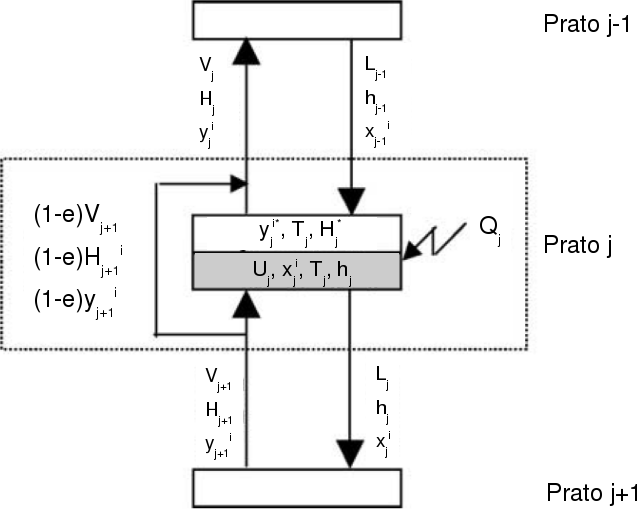
\includegraphics[scale=0.6]{images/Chap2/eficienciamurphree.png}
 \caption{Detalhes da representação de um prato segundo \citeonline{Elgue:2004}.}
 \label{fig:eficienciamurphree}
 \end{figure}

O equilíbrio termodinâmico é alcançado quando são satisfeitas as condições de equilíbrio químico, térmico e
mecânico entre as fases:
\begin{equation}
\begin{array}{c}
% \phi_{liq_i} \cdot x_{out} = \phi_{vap_i} \cdot y_{out} \\
\hat{f}^L_i = \hat{f}^V_i \qquad (i = 1,2,...,c) \\
T^L = T^V \\
P^L = P^V \\
\end{array}
\end{equation}
onde, $\hat{f}_i$ é a fugacidade da espécie ou componente $i$ em solução, o superscrito
$L$ é utilizado para o líquido e $V$ para o vapor, $T$ e $P$ são a temperatura
e a pressão, respectivamente.

\nomenclature{$\hat{f}^L_i$}{Fugacidade da espécie $i$ em solução líquida}
\nomenclature{$f^L_i$}{Fugacidade da espécie $i$, líquido puro}
\nomenclature{$\hat{f}^V_i$}{Fugacidade da espécie $i$ em solução gasosa}
\nomenclature[G]{$\gamma_i$}{Coeficiente de atividade da espécie $i$ em solução líquida}
\nomenclature[G]{$\gamma_{i,\infty}$}{Coeficiente de atividade da espécie $i$ à diluição infinita}
\nomenclature{$H_i$}{Constante de Henry da espécie $i$}

A igualdade de fugacidades, como apresentada acima, frequentemente é
representada utilizando coeficientes de fugacidade.
O coeficiente de fugacidade de um componente $i$, em uma solução gasosa, é
definido como:
\begin{equation}
\hat{\phi}^V_i \equiv \dfrac{\hat{f}^V_i}{Py_i} \qquad (i = 1,2,...,c) \\
\label{eq:phidefinition}
\end{equation}

\nomenclature[G]{$\hat{\phi}^L_i$}{Coeficiente de fugacidade da espécie $i$ em
solução líquida}
% \nomenclature{$\phi^L_i$}{Coeficiente de fugacidade da espécie $i$ pura, na fase
% % líquida}
\nomenclature[G]{$\hat{\phi}^V_i$}{Coeficiente de fugacidade da espécie $i$ em
solução gasosa}

Embora mais usual para gases, o coeficiente de fugacidade também
está definido para líquidos, pela \autoref{eq:phidefinitionL}, gerando o coeficiente $\hat{\phi}^L_i$.
\begin{equation}
\hat{\phi}^L_i \equiv \dfrac{\hat{f}^L_i}{Px_i} \qquad (i = 1,2,...,c) \\
\label{eq:phidefinitionL}
\end{equation}
Isto permite escrever a igualdade de fugacidades da seguinte forma:
\begin{equation}
\hat{\phi}^L_i x_i = \hat{\phi}^V_i y_i \qquad (i = 1,2,...,c) \\
\label{eq:phiequality}
\end{equation}
É importante notar que, embora a \autoref{eq:phiequality} envolva o
coeficiente de fugacidade, ela é geral o suficiente para tratar os casos onde
modelos de atividade são utilizados.
Isto pode ser verificado utilizando-se a definição do coeficiente de atividade
de um componente $i$ em uma solução líquida, como desvio em relação a regra de Lewis-Randall:
\begin{equation}
\gamma_i \equiv \dfrac{\hat{f}^L_i}{x_if^L_i} \qquad (i = 1,2,...,c) \\
\label{eq:gammadefinition}
\end{equation}
onde, $f^L_i$ é a fugacidade da espécie $i$ pura.

Das relações acima, é fácil demonstrar que $\hat{\phi}^L_i = \gamma_i \phi^L_i$,
com $\phi^L_i$ sendo o coeficiente de fugacidade do líquido $i$ puro, ou seja, $f^L_i = \phi^L_i P$. Assim,
para determinar o valor de $\hat{\phi}^L_i$,
basta associar um modelo de atividade (cálculo de $\gamma_i$) com uma equação de
estado (cálculo de $\phi^L_i$).
No pacote termodinâmico utilizado neste trabalho, esta é a forma de determinação
dos coeficientes de fugacidade quando modelos de atividade são utilizados.
Outra opção usual é aproximar $\phi^L_i$ como sendo simplesmente $P^{sat}_i/P$, onde
$P^{sat}_i$ é a pressão de vapor da espécie $i$ na temperatura de $T$, podendo-se ainda
fazer a correção de Poyting quando $P$ está distante de $P^{sat}_i$.

No caso de gases dissolvidos, pode-se utilizar a constante de Henry, $H_i$, associada ao coeficiente de
atividade à diluição infinita, $\gamma_{i,\infty}$, chegando-se na relação:
\begin{equation}
\hat{\phi}^L_i = \dfrac{\gamma_i H_i}{\gamma_{i,\infty} P} \qquad (i = 1,2,...,c) \\
\label{eq:gammadefinitionHenry}
\end{equation}

Neste caso, basta calcular $\phi^L_i = H_i / \gamma_{i,\infty} P$ e usar a mesma relação
$\hat{\phi}^L_i = \gamma_i \phi^L_i$.

O modelo desenvolvido neste trabalho, apresentado no \autoref{chap:moddesenvolvidos}, é baseado na condição de equilíbrio
termodinâmico.
Uma vez que o pacote de cálculo de propriedades utilizado neste trabalho
fornece os coeficientes de fugacidade independentemente do modelo termodinâmico
em uso, neste trabalho a forma apresentada na \autoref{eq:phiequality} é
preferida.

\section{Modelos de Taxa de Transferência} \label{sec:modnonequil}
% \section{Modelos de Não-Equilíbrio} \label{sec:modnonequil}
Geralmente, um estágio de separação de uma coluna de destilação é modelado com a hipótose de equilíbrio  termodinâmico
entre o vapor e o líquido existentes, mas na realidade, este equilíbrio não é alcançado. A primeira tentativa de corrigir
esta não-idealidade, ou não-equilíbrio, foi com a introdução de uma eficiência de estágio.
A eficiência de Murphree, que é um modelo de
eficiência muito utilizado, mede com que grau o equilíbrio termodinâmico é alcançado e é utilizada com certo sucesso em
sistemas binários e em estado estacionário. Porém, segundo \citeonline{Koeijer:2004}, não apresenta bons resultados
em simulações dinâmicas multicomponente.

Para explicar este desvio da idealidade no equilíbrio entre as fases, surgiu a
modelagem baseada em taxas de transferência, os chamados modelos de não-equilíbrio. De acordo com
essa corrente, a destilação é modelada por taxas de transferência que são
impulsionadas pela distância do equilíbrio e não mais pelo equilíbrio entre as
fases presentes. Nos primeiros trabalhos, as taxas de transferência foram modeladas
utilizando as equações de Maxwell-Stephan, o que acabou batizando o método
com o mesmo nome.

Assim, o método de Maxwell-Stephan se baseia na existência de um filme líquido e um filme de vapor com gradientes de
temperatura e concentração. Estes filmes entram em contato através de uma interface, onde é alcançada a condição de
equilíbrio termodinâmico entre as fases \cite{Koeijer:2004}.
% Esta estrutura pode ser vista na
% \autoref{fig:interfaceesquema}.
%  \begin{figure}[htb]
%  \centering 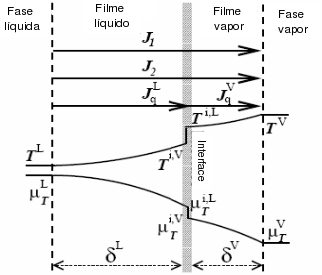
\includegraphics[scale=0.9]{images/Chap2/interfaceesquema.png}
%  \caption{Interface entre as fases líquida e vapor considerada no método de Maxwell-Stephan \cite{Koeijer:2004}}.
%  \label{fig:interfaceesquema}
%  \end{figure}

A representação esquemática global de um estágio, onde não há equilíbrio termodinâmico, pode ser vista na
\autoref{fig:nonequilibriumstage}.
 \begin{figure}[htb]
 \centering 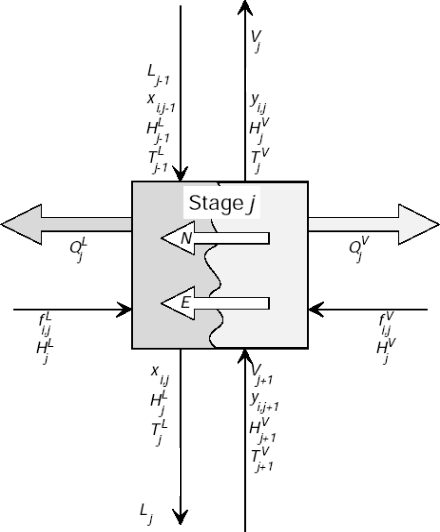
\includegraphics[scale=0.6]{images/Chap2/nonequilibriumstage.png}
 \caption{Diagrama esquemático de um estágio sem consideração de equilíbrio termodinâmico \cite{Kooijman:1995a}.}
 \label{fig:nonequilibriumstage}
 \end{figure}
A linha vertical ondulada no meio do diagrama representa a interface entre as duas fases, que podem ser tanto líquido e
vapor (no caso de um estágio de destilação) como duas fases líquidas (no caso de
um processo de extração). Estas duas fases trocam massa e energia através das
taxas $N$ e $E$, respectivamente. O força motriz destas taxas é justamente a
consideração de não-equilíbrio entre as fases.

Geralmente, o modelo de um estágio real, ou seja, sem a condição de equilíbrio, é composto por três partes. A primeira,
com as equações de balanço de massa e energia para a fase líquida, a segunda com as equações de balanço da fase vapor,
e a terceira parte, unindo as anteriores, com as equações da interface referentes às taxas de transferência de massa
e energia e a relação de equilíbrio.

Na transferência de massa, as taxas molares de líquido e vapor contam com uma contribuição difusiva e uma convectiva,
conforme a \autoref{eq:fluxomolvap} e \ref{eq:fluxomolliq}. %\autoref{eq:equilfluxomol}, 
\begin{equation}
N^V_{ij} - N^L_{ij}= 0
\label{eq:equilfluxomol}
\end{equation}
\begin{equation}
N^V_{ij} = J^V_{ij}a_j^I + y_{ij}N_{tj}
\label{eq:fluxomolvap}
\end{equation}
\begin{equation}
N^L_{ij} = J^L_{ij}a_j^I + x_{ij}N_{tj}
\label{eq:fluxomolliq}
\end{equation}
onde $a^I_j$ é a área interfacial total no estágio $j$ e $N_{tj}$ é a taxa de
transferência de massa total no estágio $j$ com $N_{tj} =
\displaystyle\sum_{i=1}^c N_{ij}$

\nomenclature{$N^V_{ij}$}{Taxa de transferência molar do componente $i$ na fase vapor, no estágio $j$ \nomunit{mol/s}}
\nomenclature{$N^L_{ij}$}{Taxa de transferência molar do componente $i$ na fase líquida, no estágio $j$ \nomunit{mol/s}}
\nomenclature{$J^V_{ij}$}{Fluxo molar difusivo do componente $i$ no vapor, no estágio $j$ \nomunit{mol/(m^2\ s)}}
\nomenclature{$J^L_{ij}$}{Fluxo molar difusivo do componente $i$ no líquido, no estágio $j$ \nomunit{mol/(m^2\ s)}}
\nomenclature{$y_{ij}$}{Fração molar no vapor do componente $i$ no estágio $j$}
\nomenclature{$x_{ij}$}{Fração molar no líquido do componente $i$ no estágio $j$}
\nomenclature{$a^I_j$}{Área interfacial total no estágio $j$ \nomunit{m^2}}
\nomenclature{$N_{tj}$}{Taxa de transferência de massa total no estágio $j$ \nomunit{mol/s}}
\nomenclature{$C_t^V$}{Concentração molar total da fase vapor \nomunit{mol/m^3}}
\nomenclature{$C_t^L$}{Concentração molar total da fase líquida\nomunit{mol/m^3}}
O fluxo difusivo $J$, na forma matricial, é dado por:
\begin{equation}
\left( J^V\right)  = C_t^V \left[ k^V\right] \left( \overline{y^V-y^I}\right) 
\label{eq:diffusionvap}
\end{equation}
\begin{equation}
\left( J^L\right)  = C_t^L \left[ k^L\right] \left( \overline{x^I-x^L}\right) 
\label{eq:diffusionliq}
\end{equation}
onde $C_t^V$ é a concentração molar total da fase vapor, $C_t^L$ é a
concentração molar total da fase líquida, $k^V$ e $k^L$ são os coeficientes de transferência de massa e
$\left( \overline{y^V-y^I}\right)$ e $\left( \overline{x^I-x^L}\right)$ são as médias das diferenças das frações
molares entre a interface e o seio da fase vapor e líquida, respectivamente.
Para o cálculo dessas diferenças, existem inúmeras teorias e correlações. Estes
cálculos geralmente dependem da geometria do prato e das condições hidráulicas do mesmo. No trabalho de
\citeonline{Hongyan:2002}, é estudado o efeito dos gradientes de concentração no prato para o cálculo da eficiência e dos
coeficientes de transferência de massa, assim como o efeito do arraste de líquido sobre estes mesmos parâmetros. Ainda
nessa linha de pesquisa, \citeonline{Kooijman:1995a} reservou um capítulo inteiro da sua tese para mostrar os
diversos modelos de dispersão existentes e novas correlações, propostas pelo autor.

\nomenclature{$C$}{Concentração molar \nomunit{mol/m^3}}
\nomenclature{$k^L$}{Coeficiente binário de transferência de massa na fase líquida \nomunit{m/s}}
\nomenclature{$k^V$}{Coeficiente binário de transferência de massa na fase vapor \nomunit{m/s}}

% A matriz dos coeficientes de transferência de massa é calculada da seguinte maneira:
% \begin{equation}
% \left[ k^P\right]  = \left[ R^P\right]^{-1} \left[ \Gamma^P\right] 
% \label{eq:matrizcoefmass}
% \end{equation}
% onde $\left[ \Gamma^P\right]$ é chamada de matriz de fatores termodinâmicos da fase P e $\left[ R^P\right]$
% à matriz das resistências à transferência de massa. Os efeitos termodinâmicos têm uma grande importância
% nesse cálculo, pois a força
% motriz fundamental da transferência de massa é o potencial químico e não o gradiente de fração molar ou de concentração.
% A matriz $\left[ \Gamma^P\right]$ deve ser calculada com modelos termodinâmicos apropriados dependendo se são utilizadas
% equações de estado ou modelos de atividade. A matriz $\left[ R^P\right]$
% leva em consideração os coeficientes binários de transferência de massa, a forma do equipamento, parâmetros operacionais
% e propriedades físicas dos componentes envolvidos. Podem ser utilizadas as equações de Maxwell-Stephan para o cálculo da
% matriz $\left[ R^P\right]$. Para um maior detalhamento destes cálculos, ver
% \citeonline{Kooijman:1995a}.

Assim como para a massa, a taxa de transferência de energia na interface é escrita:
\begin{equation}
E^V_j -  E^L_j = 0
\label{eq:balancofluxoenergia}
\end{equation}
com as taxas de transferência de energia (calor) de ambas as fases definidas por:
\begin{equation}
E^V_j = a_j^I h^V \left( T^V - T^I\right) + \sum^c_{i=1} N^V_{ij}
\overline{H}^V_{ij}
\label{eq:taxaevj}
\end{equation}
\begin{equation}
E^L_j = a_j^I h^L \left( T^I - T^L\right) + \sum^c_{i=1} N^L_{ij}
\overline{H}^L_{ij}
\label{eq:taxaelj}
\end{equation}
onde $h^V$ e $h^L$ são os coeficientes convectivos de transferência de calor na fase vapor e na fase líquida,
$T^V$, $T^I$ e $T^L$ são as
temperaturas do vapor, interface e líquido e $\overline{H}_{ij}$ é a entalpia parcial molar do componente $i$ no estágio $j$.

\nomenclature{$E^V_j$}{Taxa de transferência de energia na fase vapor no
estágio $j$ \nomunit{J/s}}
\nomenclature{$E^L_j$}{Taxa de transferência de energia na fase líquida no
estágio $j$ \nomunit{J/s}}
\nomenclature{$P^V$}{Pressão do vapor \nomunit{atm}}
\nomenclature{$P^L$}{Pressão do líquido \nomunit{atm}}
\nomenclature{$T^V$}{Temperatura do vapor \nomunit{K}}
\nomenclature{$T^L$}{Temperatura do líquido \nomunit{K}}
\nomenclature{$T^I$}{Temperatura da interface \nomunit{K}}
\nomenclature{$h^V$}{Coeficiente de transferência de calor no vapor \nomunit{J/(m^2 K s)}}
\nomenclature{$h^L$}{Coeficiente de transferência de calor no líquido \nomunit{J/(m^2\ K\ s)}}
\nomenclature{$\overline{H}_{ij}$}{Entalpia parcial molar do componente $i$ no estágio $j$ \nomunit{J/mol}}
\nomenclature{$c$}{Número de componentes}
Além das transferências de massa e energia, é adotada a condição de equilíbrio entre as fases na interface.
Vale ressaltar que o equilíbrio
termodinâmico de fases é considerado apenas na interface.

Uma grande desvantagem do modelo de não-equilíbrio é que o cálculo das taxas de
transferência requer o fornecimento de uma matriz de coeficientes de
transferência de massa, a qual necessita de dados experimentais. Infelizmente, esse
tipo de dado não está disponível em abundância na literatura, dificultando a utilização dessa modelagem.
Outro aspecto negativo é a necessidade do cálculo de propriedades de
misturas adicionais, quando comparado ao modelo de equilíbrio.
Estas propriedades adicionais são basicamente a tensão superficial,
viscosidade, condutividade térmica, além dos coeficientes de transferência de
massa.

Apesar das dificuldades, os modelos de não-equilíbrio tendem a representar a realidade de uma forma mais fidedigna que os
modelos de equilíbrio, conforme é relatado no trabalho de \citeonline{Biardi:1989} e de \citeonline{Kooijman:1995}. Por isso,
são mais utilizados para o projeto de novas unidades.

\section{Modelos Reduzidos} \label{sec:modred}
Um modelo rigoroso típico de um prato de uma coluna de destilação consiste em equações que descrevem as
concentrações das espécies, vazões de líquido e vapor, temperatura, queda de pressão e relações de
equilíbrio (ou não) entre as
fases líquida e vapor. Considerando as grandes dimensões da maioria das colunas de destilação industriais, geralmente
com mais de 50 pratos, uma simulação rigorosa do comportamento dinâmico requer a resolução de um sistema de milhares
de equações. Este procedimento de resolução pode levar um considerável tempo computacional. Nestes casos, um modelo
reduzido pode ser necessário \cite{Musch:1993}. Além disso, muitas vezes o sistema
gerado apresenta um índice diferencial elevado. O índice diferencial é utilizado como uma medida da dificuldade de
solução numérica de sistemas algébrico-diferenciais. Sistemas com índice diferencial igual a 0 são, na verdade,
sistemas de equações diferenciais ordinárias. Sistemas com índice maior que 1 são conhecidos como sistemas de índice
elevado e não podem ser tratados diretamente por códigos integradores convencionais \cite{Brennan:1989}.

Foi durante a década de 80 que os principais trabalhos a cerca da redução de modelos foram publicados. Naquela época, os
métodos de solução dos sistemas de equações gerados pela modelagem dos processos de separação eram muito limitados. Não
havia integradores de sistemas de equações algébrico-diferenciais (\emph{Differential-Algebraic Equations} - DAE), apenas
integradores para sistemas ODE (\emph{Ordinary Differential Equations}). A solução dos sistemas DAE era feita
sequencialmente, separando o sistema em um conjunto algébrico e um conjunto diferencial. Além disso, os recursos
computacionais não eram comparáveis aos oferecidos hoje, deixando as simulações ainda mais lentas.
A fim de introduzir os principais métodos utilizados na elaboração de modelos reduzidos de colunas de destilação, os
trabalhos mais relevantes encontrados na literatura são apresentados a seguir.

Em 1983, foi iniciada uma série de trabalhos sobre redução de modelos usando o método de aproximação polinomial, ou
colocação ortogonal. Quando se fala em colocação ortogonal, geralmente associa-se a uma técnica para
discretização de equações diferenciais parciais. O uso de colocação para a simulação de colunas de
destilação é uma extensão desta técnica \cite{Huss:1996}.
No trabalho de \citeonline{Cho:1984}, o procedimento de redução
de variáveis do modelo por colocação ortogonal é apresentado, este trabalho é
a base da explanação que será apresentada nos próximos parágrafos. A convenção de contagem dos pratos
adotada pelo autor é a mesma utilizada aqui e é mostrada na \autoref{fig:choejoseph}.
 \begin{figure}[htb]
 \centering 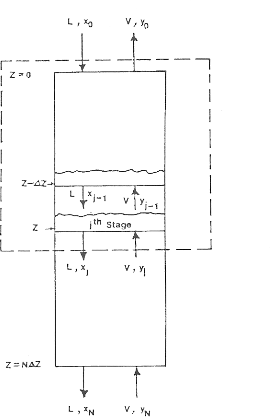
\includegraphics[scale=0.75]{images/Chap2/choejoseph.png}
 \caption{Contagem de pratos de uma coluna de destilação segundo \citeonline{Cho:1984}.}
 \label{fig:choejoseph}
 \end{figure}

Considerando a equação de balanço material em um prato de uma coluna de destilação, e considerando constantes
o acúmulo molar $M_j$ e as vazões molares $L$ e $V$, a fim de simplificação, tem-se:
\begin{equation}
M_j \dfrac{dx}{dt}=(Lx-Vy)_{j-1} - (Lx-Vy)_j \hspace{1cm} j=1,2,\ldots N
\label{eq:redbal}
\end{equation}
onde $N$ é o número de pratos da coluna. Se o perfil de concentração $x$ de uma coluna pudesse ser considerado contínuo
o mesmo poderia ser representado por:
\begin{equation}
x(z)=\sum^{n+2}_{k=1}l_k(z)x_k
\label{eq:lagrange}
\end{equation}
onde $z$ é a distância ao longo do comprimento da coluna, $l_k(z)$ são polinômios de Lagrange, $x_k$ representa o
valor de $x$ calculado em um ponto arbitrário $z_k$ e $n$ é o grau do polinômio. Reescrevendo a \autoref{eq:redbal} em termos de $z$:
\begin{equation}
M  \dfrac{dx}{dt} \mid_{z_j}=(Lx-Vy)_{z_j-\Delta z} - (Lx-Vy)_{z_j}
\label{eq:redbalz}
\end{equation}
onde $\Delta z$ é a distância entre pratos. Vale salientar que das $n+2$ equações necessárias para calcular os
$n+2$ \ $x_k$, 2 correspondem às condições de
contorno. Substituindo a \autoref{eq:lagrange} na \autoref{eq:redbalz} tem-se:
\begin{equation}
M\dfrac{dx_j}{dt}=\sum^{n+2}_{k=1} \left[ l_k(z_j-\Delta z) - l_k(z_j)\right](Lx_k-Vy_k)  \hspace{0.5cm} j=2,3,\ldots n+2
\label{eq:redbal3}
\end{equation}
\nomenclature{$M_j$}{Acúmulo molar total no estágio j \nomunit{mol}}
\nomenclature{$x$}{Fração molar no líquido}
\nomenclature{$L$}{Vazão molar de líquido\nomunit{mol/s}}
\nomenclature{$V$}{Vazão molar de vapor \nomunit{mol/s}}
\nomenclature{$N$}{Número de pratos da coluna}

Definindo:
\begin{equation}
A_{jk} = l_k(z_j-\Delta z) - l_k(z_j)
\end{equation}
com $A_{jk}$ sendo as constantes determinadas pelo grau do polinômio $n$ escolhido, a \autoref{eq:redbal3} apresenta a
forma final:
\begin{equation}
M\dfrac{dx_j}{dt}=\sum^{n+2}_{k=1} A_{jk}(Lx_k-Vy_k)  \hspace{1cm} j=2,3,\ldots n+1
\label{eq:redbalfinal}
\end{equation}
O que deve ser compreendido é a substituição das $N$ equações de balanço (\autoref{eq:redbal}) por $n$ equações
reduzidas (\autoref{eq:redbalfinal}). Escolhendo um valor de $n$ bem menor que $N$, pode-se conseguir uma enorme redução
de ordem. Por exemplo, se o perfil a ser representado é aproximadamente uma parábola, assumir $n=2$ é suficiente
independentemente do tamanho de $N$ \cite{Cho:1984}.

\nomenclature{$z$}{Distância ao longo do comprimento da coluna \nomunit{m}}
\nomenclature{$l_k(z)$}{Polinômios de Lagrange}
\nomenclature{$n$}{Grau do polinômio}
\nomenclature[G]{$\Delta z$}{Distância entre pratos \nomunit{m}}

Esta é a essência da teoria da aproximação polinomial. Para uma redução de modelo completa, este procedimento deve
ser feito com as outras equações e as outras variáveis do modelo rigoroso.

Em 1985, \citeonline{Stewart:1985} desenvolveram uma nova forma de colocação ortogonal onde as variáveis de estado de cada
estágio são aproximadas pelo polinômio de Hahn. À medida que o número de pontos de colocação se aproxima do número
de pratos reais do sistema a resposta da redução se aproxima à resposta do sistema completo, isto é, a maior
ordem de aproximação permitida pelo método é um ponto de colocação por estágio.
A importância deste trabalho é mostrada em uma comparação do método desenvolvido com outros métodos de redução, segundo
critérios de avaliação estabelecidos. Esta comparação mostra que a colocação utilizando polinômios de Hahn
é a mais adequada para sistemas de separação por estágios segundo todos os
quesitos de avaliação estudados.

Partindo do trabalho de \citeonline{Stewart:1985}, \citeonline{Pinto:1988} testaram novas
estratégias de redução de modelos e analisaram diferentes famílias de polinômios ortogonais
para esta aplicação. As principais contribuições sobre os trabalhos anteriores está na
constatação de que o prato de alimentação assim como as extremidades da coluna (condensador
e refervedor) devem ser considerados como pontos
de colocação e interpolação para que a redução do modelo apresente melhores resultados.
Além disso, polinômios ortogonais diferentes dos usuais (Lagrange, Jacobi e Hahn) foram gerados e utilizados para a redução com sucesso.

\apudonline{Benallou:1986}{Musch:1993} propuseram um importante método de redução de modelos baseado em modelos
compartimentais. Estes modelos fazem uso do fato de que pratos adjacentes apresentam pequenas diferenças de vazões
e temperaturas, podendo assim serem agrupados em ``compartimentos''. Balanços de massa e energia e relações
hidrodinâmicas são especialmente desenvolvindos para esses blocos, onde apenas um prato é modelado, sendo este o
\textit{prato referência} do bloco. São adotadas também, variações uniformes de temperatura, vazões e pressões dentro
dos compartimentos, assim como relações algébricas entre as composições que saem de cada bloco.

Buscando aperfeiçoar o método de \citeonline{Benallou:1986} e sanar algumas desvantagens apresentadas pelas suas
simplificações, \citeonline{Musch:1993} realizaram algumas modificações no modelo original, que foram: substituição da
eficiência de vaporização pela eficiência de Murphree; adição de equações diferenciais de
balanço de componente em substituição às relações algébricas de concentração. As principais simplificações deste modelo,
em relação a um modelo rigoroso completo de coluna de destilação são:
\begin{itemize}
\item todos os pratos de um mesmo bloco possuem o mesmo acúmulo;
\item as vazões de líquido e vapor dentro de um compartimento são uniformes;
\item o perfil de temperatura entre os pratos adjacentes ao prato de referência é linear;
\item a queda de pressão em cada prato de um bloco é igual à queda de pressão no prato referência do mesmo compartimento.
\end{itemize}

Com estas simplificações, este modelo reduzido contém as seguintes equações:
\begin{itemize}
\item Por prato:
	\begin{itemize}
	\item (número de componentes - 1) equações diferenciais de balanço de massa;
	\item (número de componentes) equações de relação de equilíbrio entre as fases.
	\end{itemize}
\item Por bloco, isto é, por compartimento:
	\begin{itemize}
	\item uma equação diferencial de balanço de massa global;
	\item uma equação de balanço de energia;
	\item uma equação para o cálculo da vazão de líquido e uma equação para o cálculo da vazão de vapor;
	\item uma equação de cálculo da queda de pressão;
	\item uma equação de interpolação do perfil de temperatura.
	\end{itemize}
\end{itemize}

A precisão da resposta deste modelo depende intimamente do número de blocos em que a coluna é reduzida. Quanto maior a
divisão, isto é, quanto maior o número de compartimentos, mais o modelo se aproxima de um modelo rigoroso.

Outra forma de redução do modelo é apresentada no trabalho de \citeonline{Osorio:2004}, com 
a substituição do sistema de equações algébrico-diferencial (DAE) por um sistema de
equações diferenciais ordinárias (ODE). As equações algébricas, principalmente as referentes ao equilíbrio das fases, são
substituídas por uma rede neuronal previamente ajustada com dados experimentais. Para a realização deste ajuste
é necessário uma grande quantidade de dados experimentais. Segundo os autores, esta mescla de modelagem rigorosa com modelos
empíricos reduz o tempo de simulação em até 40\%. Apesar da maior eficiência, modelos empíricos
não podem ser utilizados para predições fora da faixa de dados com os quais foram ajustados, o que limita sua
capacidade de extrapolação.

Muitos outros trabalhos com diferentes aplicações ou diferentes metodologias de redução foram encontrados
na literatura, entre eles estão: \citeonline{Betlem:2000} e \citeonline{Diwekar:1987} com aplicação de modelos
reduzidos em colunas de destilação batelada e a série de trabalhos de \citeauthor{Srivastava:1985} que
mostraram que o grau de redução do
modelo alcançável depende da natureza do perfil de composição e apresentaram novas
metodologias para ultrapassar esta limitação.

Por mais que os modelos reduzidos tenham uma boa precisão, tanto da dinâmica do sistema quanto do resultado estacionário,
estes não substituem os modelos rigorosos. Os modelos de baixa ordem são principalmente utilizados em aplicações onde é
necessária a realização de simulações repetitivamente, como em otimização de processos ou em estudos de sínteses de
sistemas de controle \cite{Cho:1984}.


% \section{Modelos com previsão de duas fases líquidas} \label{sec:VLL}
% Na modelagem de uma destilação com a presença de duas fases (Vapor-Líquido) apenas uma interface é identificada, conforme
% visto na \autoref{sec:modnonequil}. Porém, em uma destilação com duas fases líquidas e uma vapor (V-L1-L2) três
% interfaces são encontradas.
% 
% De acordo com \citeonline{Eckert:2001}, as fases líquidas apresentam comportamentos diferentes: a fase em maior
% quantidade é considerada um líquido contínuo (LC) enquanto a outra, menos abundante, encontra-se presente na forma de
% gotas dispersas na fase contínua, sendo denominada de fase dispersa (LD). A \autoref{fig:vllesquema} ilustra esse
% comportamento.
%  \begin{figure}[htb]
%  \centering 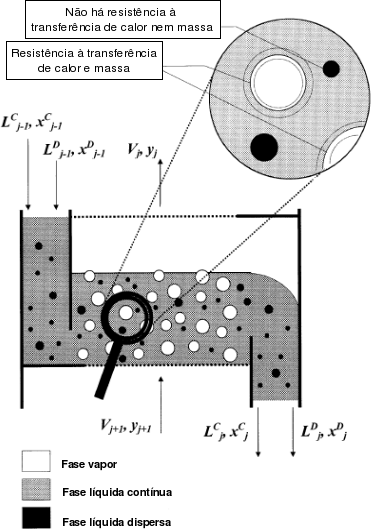
\includegraphics[scale=0.7]{images/Chap2/vllesquema.png}
%  \caption{Esquema simplificado de um estágio com três fases V-L1-L2 \cite{Eckert:2001}.}
%  \label{fig:vllesquema}
%  \end{figure}
% 
% A destilação com formação de mais de uma fase líquida pode ser resolvida de diversas maneiras. Pode-se assumir a condição
% de não-equilíbrio entre todas as fases, ou apenas entre a fase líquida em maior quantidade e o vapor, ou ainda pode-se
% ignorar a modelagem de não-equilíbrio e considerar o equilíbrio termodinâmico entre todas as fases.
% 
% \citeonline{Eckert:2001} adotaram algumas
% considerações para simplificar a modelagem. Dentre as principais estão: a) as duas fases líquidas estão em equilíbrio
% termodinâmico e b) a fase dispersa (LD) e a fase vapor não entram em contato.
% Com estas simplificações, os autores formularam um modelo com a combinação de equações de não-equilíbrio entre a
% fase líquida contínua (LC) e o vapor, e equações com condição de equilíbrio entre as duas fases líquidas.
% 
% Já no trabalho de \citeonline{Eckert:1995} apenas relações de equilíbrio entre as fases foram consideradas. A modelagem
% proposta suporta o aparecimento de mais de duas fases líquidas com uma fase vapor. As equações de equilíbrio são descritas
% da seguinte maneira:
% \begin{equation}
% \begin{array}{ll}
% y_{i,j} = K^r_{i,j} x^r_{i,j}  & i=1,\ldots,c; j=1,\ldots,N \\
% K^r_{i,j} x^r_{i,j} = K^k_{i,j} x^k_{i,j} & k=1,\ldots,p; k\neq r
% \end{array}
% \label{eq:equilibriol}
% \end{equation}
% onde o índice $r$ se refere a uma fase líquida escolhida como referência e o índice $p$ ao número de fases líquidas que
% podem aparecer no sistema.
% 
% Vale ressaltar que em sistemas V-L1-L2, tão importante quanto o grau de fidelidade da modelagem é a qualidade dos modelos
% termodinâmicos utilizados, principalmente na predição do equilíbrio entre duas fases líquidas, onde as equações cúbicas
% de estado não podem ser utilizadas. Sabe-se da dificuldade de obtenção dos parâmetros empíricos necessários para o
% cálculo dos coeficientes de atividade, seja qual for o modelo utilizado. Segundo \citeonline{Suppes:2002}, para sistemas
% que envolvam equilíbrio com mais de uma fase líquida, devem ser utilizadas as equações NRTL ou TK Wilson.
% 
% \nomenclature{$K_i$}{Razão de equilíbrio do componente $i$: $K_i=y_i/x_i$}

\section{Considerações Finais}

Como visto neste capítulo, o aumento da precisão na predição de um modelo é
acompanhado pelo crescimento da sua complexidade e, consequentemente, dos
recursos computacionais necessários para resolvê-lo. Isto significa que o grau de fidelidade do modelo
utilizado deve assumir um compromisso entre a simplicidade e a precisão para
evitar problemas numéricos e ser computacionalmente viável
\cite{Klingberg:2000}.
Além disso, modelos muito rigorosos podem envolver um grande número de
parâmetros, que podem acabar por inserir incertezas.

A escolha das considerações simplificativas varia com a aplicação do modelo.
Em estudos onde são necessárias simulações repetitivas, como em otimizações,
os modelos reduzidos podem ser os indicados. Mas em estudos de partidas e
paradas de colunas de destilação é importante que o comportamento dinâmico do
sistema seja bem representado levando ao uso de modelos rigorosos completos.

%
%
%
\chapter{Modelagem Matemática} \label{chap:moddesenvolvidos}


\emph{Modelos matemáticos de colunas de destilação podem ser classificados de acordo com o seu grau de detalhamento:
se possuem predição da composição, temperatura e vazões para cada prato, são chamados de modelos rigorosos. Se são
compostos por uma descrição global da coluna utilizando um menor número de variáveis, baseados em algum tipo de
interpolação, são ditos modelos reduzidos \cite{Fletcher:2000}. Neste trabalho, os modelos desenvolvidos fazem parte do
primeiro
grupo, modelos rigorosos, prato-a-prato, baseados na consideração de equilíbrio termodinâmico entre as fases líquida e
vapor.
}

\section{Introdução}

Para o desenvolvimento de um modelo de coluna de destilação, diversos modelos
de equipamentos periféricos são necessários. Exemplos destes equipamentos são:
bomba, válvula, tanques, condensador e referverdor.
Neste capítulo, os modelos desenvolvidos são apresentados, com suas
considerações e equacionamento.

Além dos modelos dos equipamentos individuais, é apresentado um estudo a
respeito de correlações hidráulicas disponíveis na literatura para o cálculo
das vazões internas da coluna.

Para a implementação dos modelos e simulações foi utilizado o software \emso\
(\emsoname) que é uma ferramenta de modelagem, simulação e
otimização de processos.
O simulador \emso\ pode ser utilizado de forma genérica e nos mais variados
ramos da engenharia. Apresenta várias características importantes que auxiliam
no desenvolvimento de modelos e na realização de simulações como: análise de
consistência de unidades de medida, verificação de singularidades do sistema e
consistência das condições iniciais. Mais detalhes sobre o simulador são
apresentados no \autoref{ap:emso} desta dissertação.

% Um sistema de separação, como por exemplo uma coluna de destilação, é formado por um conjunto de equipamentos. Para cada
% um dos equipamentos mais comuns encontrados nesse tipo de sistema foram confeccionados modelos que tentam prever o
% comportamento dinâmico e$\setminus$ou estacionário dos mesmos. Estes modelos serão apresentados a seguir nas próximas
% seções.

% \section{Bomba e Divisor de correntes}

\section{Bomba} \label{sec:modelobomba}
Neste trabalho um modelo simplificado de bomba foi construído.
Este modelo é utilizado apenas para reintroduzir na coluna de destilação a corrente de destilado em uma pressão maior
que a do prato do topo. Desta forma, este modelo inclui apenas um acréscimo de pressão da sua corrente de saída com
relação à corrente de entrada.
Sua representação esquemática pode ser vista na \autoref{fig:esquemapump}:

\begin{figure}[htb]
\centering 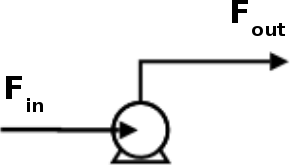
\includegraphics[scale=0.5]{images/Chap3/esquemapump2.png}
\caption{Modelo esquemático de uma bomba}
\label{fig:esquemapump}
\end{figure}

Trata-se de um modelo simplificado, onde o usuário fornece uma queda de pressão $\Delta P$ e é composto pelas equações:

\begin{flushleft}
Balanço de massa:
\end{flushleft}
\begin{equation}
F_{in} = F_{out}
\end{equation}
\begin{equation}
z_{in_i} = z_{out_i}  \qquad i=1,2,\cdots,c
\end{equation}
\nomenclature{$F_{in}$}{Vazão molar que entra no equipamento \nomunit{mol/s}}
\nomenclature{$F_{out}$}{Vazão molar que sai do equipamento \nomunit{mol/s}}
\nomenclature{$z_{in}$}{Vetor de frações molares dos componentes da corrente que entra no equipamento}
\nomenclature{$z_{out}$}{Vetor de frações molares dos componentes da corrente que sai do equipamento}
\nomenclature{$z_{in_i}$}{Fração molar do componente $i$ na corrente que entra no equipamento}
\nomenclature{$z_{out_i}$}{Fração molar do componente $i$ na corrente que sai do equipamento}
Pressão:
\begin{equation}
P_{out} = P_{in} + \Delta P
\end{equation}
\nomenclature{$P_{out}$}{Pressão da corrente que sai do equipamento \nomunit{atm}}
\nomenclature{$P_{in}$}{Pressão da corrente que entra do equipamento \nomunit{atm}}
% \nomenclature{$dP$}{Queda de pressão no equipamento ($atm$)}
Entalpia:
\begin{equation}
h_{out} = h_{in} + \dfrac{\Delta P}{\rho} \cdot Mw
\end{equation}
Massa Específica:
\begin{equation}
\dfrac{1}{\rho} = \dfrac{(1-v)}{\rho^L} + \dfrac{v}{\rho^V}
\end{equation}
% onde as composições das fases líquida e vapor na saída da bomba, necessárias para o cálculo da fração
% vaporizada e das propriedades físicas são obtidas através da solução de um \textit{flash PH}.
onde $Mw$ é a massa molar média da mistura, $v$ é a fração vaporizada da corrente, $\rho$ é a massa específica e
os superscritos $L$ e $V$ são utilizados para especificar o caso líquido e
vapor, respectivamente.

Adicionalmente às equações acima, a temperatura e a fração
vaporizada da corrente que sai da bomba são calculadas pelo pacote
termodinâmico através de um cálculo de \textit{flash}.
Isto é necessário para
que todas as informações da corrente de saída da bomba estejam disponíveis, permitindo que esta seja conectada
a qualquer outro modelo desenvolvido no EMSO.
Isto poderá ser visualizado mais adiante, quando for construído o modelo de uma
coluna de destilação completa.

\nomenclature{$T_{out}$}{Temperatura da corrente que sai do equipamento \nomunit{K}}
\nomenclature{$T_{in}$}{Temperatura da corrente que entra do equipamento \nomunit{K}}
\nomenclature[G]{$\rho$}{Massa específica da corrente \nomunit{kg/m^3}}

Na linguagem do simulador \emso\ o modelo acima apresentado pode ser escrito
conforme o \autoref{code:bomba}: \lstinputlisting[firstline=3, lastline=33, numbers=none, language=EMSO, caption=Modelo simplificado de bomba. , label=code:bomba] {images/Chap4/pump.mso}

Deve-se ficar atento ao fato de que, em algumas equações, se faz uso de funções externas ao simulador, no caso
funções de \textit{plugins}. No \autoref{code:bomba}, isto acontece no cálculo da massa específica, onde a
densidade da mistura na fase líquida e na fase vapor são calculadas através de funções do \textit{plugin} PP
que foi previamente declarado na seção de parâmetros. Este \textit{plugin} consiste é um pacote termodinâmico
que realiza os cálculos de propriedades físicas e termodinâmicas da mistura a ser simulada. Praticamente todos os
modelos apresentados aqui necessitam de alguma cálculo deste tipo.


\section{Divisor de correntes: \textit{splitter}} \label{sec:modelosplitter}
\textit{Splitter} é um divisor de correntes, utilizado em modelos de colunas de destilação para separar a corrente
de topo em destilado e refluxo e para separar o produto de fundo da corrente que volta para
o refervedor.

Um \textit{splitter} pode ser representado pela \autoref{fig:splitter}, onde a corrente de entrada se
separa em duas correntes de saída. Um parâmetro fixado pelo usuário, chamado $frac$, determina qual proporção da vazão de
entrada vai para a corrente $out1$.
\begin{figure}[htb]
\centering 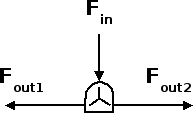
\includegraphics[scale=0.9]{images/Chap3/esquemasplitter2.png}
\caption{Modelo esquemático de um \textit{splitter}}
\label{fig:splitter}
\end{figure}

O modelo do \textit{splitter} é composto pelas seguintes equações:

\begin{flushleft}
Vazão:
\end{flushleft}
\begin{equation}
F_{out1} = F_{in} \cdot frac
\end{equation}
\begin{equation}
F_{out2} + F_{out1} = F_{in}
\end{equation}
\nomenclature{$frac$}{Fração de \textit{split} da vazão}
Temperatura:
\begin{equation}
T_{out1} = T_{in}
\end{equation}
\begin{equation}
T_{out2} = T_{in}
\end{equation}
Pressão:
\begin{equation}
P_{out1} = P_{in}
\end{equation}
\begin{equation}
P_{out2} = P_{in}
\end{equation}
Composição:
\begin{equation}
z_{out1_i} = z_{in_i} \qquad i=1,2,\cdots,c
\end{equation}
\begin{equation}
z_{out2_i} = z_{in_i} \qquad i=1,2,\cdots,c
\end{equation}
Entalpia:
\begin{equation}
h_{out1} = h_{in} \quad\textrm{ou}\quad h_{out1} = h(T_{out1}, P_{out1},
z_{out1})
\end{equation}
\begin{equation}
h_{out2} = h_{in} \quad\textrm{ou}\quad h_{out2} = h(T_{out2}, P_{out2},
z_{out2})
\end{equation}
Fração Vaporizada da corrente:
\begin{equation}
v_{out1} = v_{in} \quad\textrm{ou}\quad v_{out1} = v(T_{out1}, P_{out1},
z_{out1})
\end{equation}
\begin{equation}
v_{out2} = v_{in} \quad\textrm{ou}\quad v_{out2} = v(T_{out2}, P_{out2},
z_{out2})
\end{equation}
\nomenclature{$h_{out}$}{Entalpia da corrente que sai do equipamento \nomunit{J/mol}}
\nomenclature{$h_{in}$}{Entalpia da corrente que entra no equipamento \nomunit{J/mol}}

No \autoref{code:splitter}, pode-se ver a implementação do equacionamento acima
na linguagem do simulador \emso.
\lstinputlisting[firstline=68, lastline=96, numbers=none, language=EMSO, caption=Modelo de \textit{splitter}. ,
label=code:splitter] {images/Chap4/splitter.mso}

\section{Tanques de acúmulo}
Os tanques são responsáveis pelo acúmulo da maior parte da mistura que
se encontra no interior da coluna de destilação.
Neste trabalho, dois modelos foram desenvolvidos, apresentados a seguir.

\subsection{Tanque cilíndrico vertical} \label{sec:modelotanquecilindrico}
Neste trabalho o modelo dinâmico de um tanque cilíndrico vertical, como
representado na \autoref{fig:esquematank1}, foi construído.
Esse modelo considera apenas uma fase líquida misturada perfeitamente e que não
há perda de carga no bocal de alimentação.
Esse modelo é geralmente utilizado acoplado abaixo do prato de fundo da coluna, quando um refervedor termossifão é utilizado.

\begin{figure}[htb]
\centering 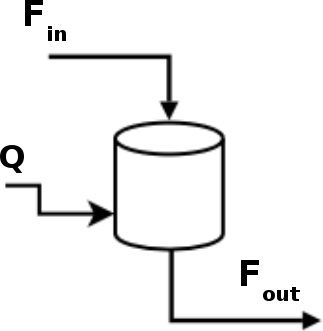
\includegraphics[scale=0.5]{images/Chap3/esquematank2.png}
\caption{Modelo esquemático de um tanque cilíndrico.}
\label{fig:esquematank1}
\end{figure}
O modelo é composto pelas seguintes equações:

\begin{flushleft}
Balanço molar por componente:
\end{flushleft}
\begin{equation}
\dfrac{dM_i}{dt} = F_{in} \cdot z_{in_i} - F_{out}  \cdot z_{out_i} \qquad i=1,2,\cdots,c
\end{equation}
% \nomenclature{$M$}{Acúmulo molar total ($mol$)}
\nomenclature{$M_i$}{Acúmulo molar do componente $i$ \nomunit{mol}}
\nomenclature{$M_k$}{Acúmulo molar do componente $k$ \nomunit{mol}}
Balanço de energia:
\begin{equation}
\dfrac{dE}{dt} = F_{in} \cdot h_{in} - F_{out}  \cdot h_{out} + Q
\end{equation}
\nomenclature{$E$}{Energia interna do sistema \nomunit{J}}
\nomenclature{$Q$}{Taxa de calor \nomunit{J/s}}
Acúmulo de energia:
\begin{equation}
E = \sum_i M_i \cdot h_{out}
\end{equation}
Relação entre acúmulos e composições:
\begin{equation}
M_i = z_{out_i} \cdot \sum_k M_k \qquad i=1,2,\cdots,c
\end{equation}
Sem perda de carga:
\begin{equation}
P_{out} = P_{in}
\end{equation}
Nível de líquido:
\begin{equation}
Level = \dfrac{\sum_i M_i \cdot v^L}{A_{cross}}
\end{equation}
\nomenclature{$v^L$}{Volume molar da fase líquida \nomunit{m^3/mol}}
\nomenclature{$v^V$}{Volume molar da fase vapor \nomunit{m^3/mol}}
\nomenclature{$v$}{Fração vaporizada da corrente}
\nomenclature{$Level$}{Nível de líquido \nomunit{m}}
\nomenclature{$A_{cross}$}{Área da seção transversal \nomunit{m^2}}

As propriedades físicas e termodinâmicas necessárias são calculadas através de rotinas externas,
baseadas no modelo termodinâmico adotado:
\begin{equation}
h_{out} = h(T_{out}, P_{out}, z_{out})
\end{equation}
\begin{equation}
v^L = v^L(T_{out}, P_{out}, z_{out})
\end{equation}

Na linguagem do simulador \emso\ o modelo acima apresentado assume a forma
mostrada no \autoref{code:tanquedepe}.
\lstinputlisting[firstline=10, lastline=49, numbers=none, language=EMSO, caption=Modelo de tanque de acúmulo. ,
label=code:tanquedepe] {images/Chap4/tank.mso}

\subsection{Tanque cilíndrico horizontal} \label{sec:modelotanquecilindrodeitado}
Este modelo se baseia nas mesmas considerações do modelo de tanque vertical,
porém apresenta a geometria de um cilindro deitado, como pode ser visto na \autoref{fig:esquematank2}:
\begin{figure}[htb]
\centering 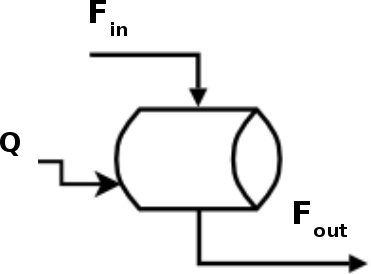
\includegraphics[scale=0.5]{images/Chap3/esquematank_22.png}
\caption{Modelo esquemático de um tanque cilíndrico deitado.}
\label{fig:esquematank2}
\end{figure}

No processo estudado no \autoref{chap:coldeiso}, este equipamento é utilizado no
topo da coluna, pois a dinâmica do condensador é muito rápida.
Nestes casos, este tanque serve como um pulmão para as bombas do refluxo e destilado.
Nos casos em que a dinâmica do condensador é muito rápida usualmente um modelo estacionário é utilizado,
como apresentado na \autoref{sec:modelocondensadorestacionario}.
Um modelo dinâmico de tanque cilíndrico horizontal pode ser composto pelas seguintes equações:

\begin{flushleft}
Balanço molar por componente:
\end{flushleft}
\begin{equation}
\dfrac{dM_i}{dt} = F_{in} \cdot z_{in_i} - F_{out}  \cdot z_{out_i}  \qquad i=1,2,\cdots,c
\end{equation}
Balanço de energia:
\begin{equation}
\dfrac{dE}{dt} = F_{in} \cdot h_{in} - F_{out}  \cdot h_{out} + Q
\end{equation}
Acúmulo de energia:
\begin{equation}
E = \sum_i M_i \cdot h_{out}
\end{equation}
Relação entre acúmulos e composições:
\begin{equation}
M_i = z_{out_i} \cdot \sum_j M_j \qquad i=1,2,\cdots,c
\end{equation}
Sem perda de carga:
\begin{equation}
P_{out} = P_{in}
\end{equation}
Área da seção transversal do cilindro deitado:
\begin{equation}
A_{cross} = r^2 \cdot \left( asin(1) - asin(\dfrac{r-Level}{r}) \right)  + (Level-r) \cdot \sqrt{Level \cdot (2 \cdot r - Level)}
\end{equation}
\nomenclature{$r$}{Raio \nomunit{m}}
\nomenclature{$L$}{Comprimento do tanque \nomunit{m}}
Acúmulo de líquido:
\begin{equation}
A_{cross} \cdot L = \sum_i M_i \cdot v^L
\end{equation}
As propriedades físicas e termodinâmicas necessárias são calculadas através de rotinas externas:
\begin{equation}
h_{out} = h(T_{out}, P_{out}, z_{out})
\end{equation}
\begin{equation}
v^L = v^L(T_{out}, P_{out}, z_{out})
\end{equation}
Este equacionamento, implementado no \emso, apresenta a seguinte estrutura
mostrada no \autoref{code:tanquedeitado}.
\lstinputlisting[firstline=50, lastline=95, numbers=none, language=EMSO, caption=Modelo de tanque cilíndrico deitado. ,
label=code:tanquedeitado] {images/Chap4/tank.mso}

\section{Refervedores}
Dois modelos de refervedor foram desenvolvidos: um modelo dinâmico, representando um refervedor do tipo
\textit{Kettle}; e um modelo estacionário correspondendo a um refervedor termossifão.

\subsection{Refervedor Dinâmico} \label{sec:modelorefervedordinamico}
O refervedor dinâmico aqui modelado pode ser representado pela \autoref{fig:esquemarebdin}. Como pode ser visto, o
refervedor recebe uma corrente de alimentação, no caso de destilações batelada, e uma corrente de líquido
proveniente da coluna. Possui como
saída duas correntes, uma líquida e outra vapor. Este refervedor é considerado como mais um estágio de
equilíbrio da coluna, em condição de mistura perfeita em ambas as fases.

\begin{figure}[htb]
\centering 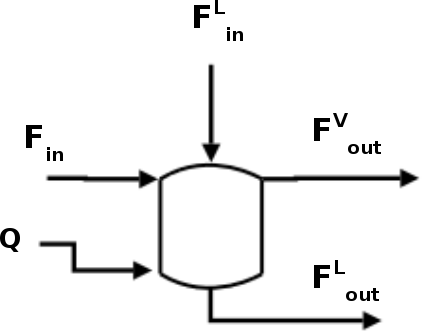
\includegraphics[scale=0.5]{images/Chap3/esquemareboiler2.png}
\caption{Modelo esquemático de um refervedor dinâmico.}
\label{fig:esquemarebdin}
\end{figure}

O modelo é composto pelas seguintes equações:

% \begin{flushleft}
Balanço molar por componente:
% \end{flushleft}
\begin{equation}
\dfrac{dM_i}{dt} = F_{in} \cdot z_{in_i} + F_{in}^L \cdot x_{in_i}- F_{out}^L  \cdot x_{out_i} - F_{out}^V \cdot y_{out_i} \qquad i=1,2,\cdots,c
\end{equation}
\nomenclature{$F_{in}^L$}{Vazão molar de líquido que entra no equipamento \nomunit{mol/s}}
\nomenclature{$F_{out}^L$}{Vazão molar de líquido que sai do equipamento \nomunit{mol/s}}
\nomenclature{$F_{out}^V$}{Vazão molar de vapor que sai do equipamento \nomunit{mol/s}}
\nomenclature{$F_{in}^V$}{Vazão molar de vapor que entra no equipamento \nomunit{mol/s}}
\nomenclature{$x_{in}$}{Vetor de frações molares dos componentes da corrente de líquido que entra no equipamento}
\nomenclature{$x_{in_i}$}{Fração molar do componente \textit{i} na corrente de líquido que entra no equipamento}
\nomenclature{$x_{out}$}{Vetor de frações molares dos componentes da corrente de líquido que sai do equipamento}
\nomenclature{$x_{out_i}$}{Fração molar do componente \textit{i} na corrente de líquido que sai do equipamento}
\nomenclature{$y_{in}$}{Vetor de frações molares dos componentes da corrente de vapor que entra no equipamento}
\nomenclature{$y_{in_i}$}{Fração molar do componente \textit{i} na corrente de vapor que entra no equipamento}
\nomenclature{$y_{out}$}{Vetor de frações molares dos componentes da corrente  de vapor que sai do equipamento}
\nomenclature{$y_{out_i}$}{Fração molar do componente \textit{i} na corrente de vapor que sai do equipamento}
Balanço de energia:
\begin{equation}
\dfrac{dE}{dt} = F_{in} \cdot h_{in} + F_{in}^L \cdot h_{in}^L - F_{out}^L  \cdot h_{out}^L - F_{out}^V \cdot h_{out}^V + Q
\end{equation}
\nomenclature{$h_{out}^L$}{Entalpia da corrente de líquido que sai do equipamento \nomunit{J/mol}}
\nomenclature{$h_{out}^V$}{Entalpia da corrente de vapor que sai do equipamento \nomunit{J/mol}}
\nomenclature{$h_{in}^L$}{Entalpia da corrente de líquido que entra no equipamento \nomunit{J/mol}}
\nomenclature{$h_{in}^V$}{Entalpia da corrente de vapor que entra no equipamento \nomunit{J/mol}}
Acúmulos:
\begin{equation}
M_i = M^L \cdot x_{out_i} + M^V \cdot y_{out_i} \qquad i=1,2,\cdots,c
\end{equation}
\begin{equation}
E = M^L \cdot h_{outL} + M^V \cdot h_{outV} - P_{out}^L \cdot V_{ref}
\end{equation}
\nomenclature{$M^L$}{Acúmulo molar de líquido \nomunit{mol}}
\nomenclature{$M^V$}{Acúmulo molar de vapor \nomunit{mol}}
\nomenclature{$V_{ref}$}{Volume do refervedor \nomunit{m^3}}
Restrições das frações molares:
\begin{equation}
\sum_i x_{out_i} = 1
\end{equation}
\begin{equation}
\sum_i x_{out_i} = \sum_i y_{out_i}
\end{equation}
Equilíbrio químico, mecânico e térmico:
\begin{equation}
\hat{\phi}_i^L \cdot x_{out_i} = \hat{\phi}_i^V \cdot y_{out_i} \qquad i=1,2,\cdots,c
\end{equation}
\begin{equation}
P_{out}^L = P_{out}^V
\end{equation}
\begin{equation}
T_{out}^L = T_{out}^V
\end{equation}
\nomenclature[G]{$\phi_i^L$}{Coeficiente de fugacidade da espécie $i$, líquido puro}
\nomenclature[G]{$\phi_i^V$}{Coeficiente de fugacidade da espécie $i$, vapor puro}
Restrição geométrica:
\begin{equation}
V_{ref} = M^L \cdot v^L + M^V \cdot v^V 
\end{equation}
Nível de líquido:
\begin{equation}
Level = \dfrac {M^L \cdot v^L}{A_{cross}}
\end{equation}

As propriedades físicas e termodinâmicas necessárias são calculadas através de rotinas externas:
\begin{equation}
h_{out}^L = h^L(T_{out}^L, P_{out}^L, x_{out})
\end{equation}
\begin{equation}
h_{out}^V = h^V(T_{out}^V, P_{out}^V, y_{out})
\end{equation}
\begin{equation}
v^L = v^L(T_{out}^L, P_{out}^L, x_{out})
\end{equation}
\begin{equation}
v^V = v^V(T_{out}^V, P_{out}^V, y_{out})
\end{equation}
\begin{equation}
\hat{\phi}_i^L = \hat{\phi}_i^L(T_{out}^L, P_{out}^L, x_{out}) \qquad
i=1,2,\cdots,c
\end{equation}
\begin{equation}
\hat{\phi}_i^V = \hat{\phi}_i^V(T_{out}^V, P_{out}^V, y_{out}) \qquad
i=1,2,\cdots,c
\end{equation}
\begin{equation}
\rho^V = \rho^V(T_{out}^V, P_{out}^V, y_{out})
\end{equation}
\nomenclature[G]{$\rho^V$}{Massa específica da fase vapor \nomunit{kg/m^3}}
\nomenclature[G]{$\rho^L$}{Massa específica da fase líquida\nomunit{kg/m^3}}

O modelo do refervedor dinâmico, na linguagem do \emso, é apresentado no
\autoref{code:refervedordinamico}.

\lstinputlisting[firstline=48, lastline=115, numbers=none, language=EMSO, caption=Modelo de refervedor dinâmico. ,
label=code:refervedordinamico] {images/Chap4/reboiler.mso}

\subsection{Refervedor Estacionário} \label{sec:modelorefervedorestacionario}
O modelo apresentado a seguir representa um refervedor estacionário e total. Segundo o equacionamento, o equipamento
recebe uma corrente líquida que é vaporizada totalmente. Não há condição de equilíbrio termodinâmico entre as fases. O
desenho esquemático pode ser visto na \autoref{fig:reboilersteady}:
\begin{figure}[htb]
\centering 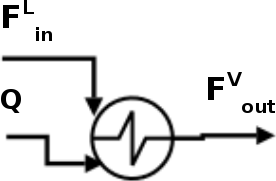
\includegraphics[scale=0.5]{images/Chap3/esquemareboilersteady2.png}
\caption{Modelo esquemático de um refervedor estacionário.}
\label{fig:reboilersteady}
\end{figure}

O modelo é composto pelas seguintes equações:

\begin{flushleft}
Balanço de massa:
\end{flushleft}
\begin{equation}
F_{in}^L = F_{out}^V
\end{equation}
\begin{equation}
x_{in_i} = y_{out_i} \qquad i=1,2,\cdots,c
\end{equation}
Balanço de energia:
\begin{equation}
F_{in}^L \cdot h_{in}^L + Q= F_{out}^V \cdot h_{out}^V 
\end{equation}
Queda de pressão:
\begin{equation}
\Delta P = P_{in}^L - P_{out}^V
\end{equation}
As propriedades físicas e termodinâmicas necessárias são calculadas através de rotinas externas:
\begin{equation}
h_{out}^L = h^L(T_{out}^L, P_{out}^L, x_{out})
\end{equation}
\begin{equation}
h_{out}^V = h^V(T_{out}^V, P_{out}^V, y_{out})
\end{equation}
\begin{equation}
v^V = v^V(T_{out}^V, P_{out}^V, y_{out})
\end{equation}
\begin{equation}
\rho^V = \rho^V(T_{out}^V, P_{out}^V, y_{out})
\end{equation}

A implementação do modelo na linguagem do simulador \emso\ é apresentada no
\autoref{code:refervedorestacionario}.
\lstinputlisting[firstline=119, lastline=149, numbers=none, language=EMSO, caption=Modelo de refervedor estacionário. ,
label=code:refervedorestacionario] {images/Chap4/reboiler.mso}

\section{Condensadores}
Colunas de destilação podem possuir vários tipos de condensadores e
refervedores.
Em alguns casos, os condensadores possuem um acúmulo significativamente
maior que o acúmulo dos pratos. Este fato contribui para uma maior estabilidade
operacional do equipamento.
Esta variedade de configurações leva a
diferentes comportamentos dinâmicos e exerce um grande efeito no comportamento da coluna \cite{Kooijman:1995a}.

Neste trabalho, dois modelos de condensadores foram construídos: um modelo
dinâmico em equilíbrio termodinâmico, representando um condensador parcial;
e um modelo estacionário com condensação total, que pode ser integrado a um modelo de tanque
de acúmulo para o comportamento dinâmico.

\subsection{Condensador Dinâmico ou Parcial} \label{sec:modelocondensadordinamico}
Na literatura, são encontrados modelos tradicionais e consolidados deste tipo de equipamento. Geralmente o condensador
dinâmico é
modelado como mais um estágio de equilíbrio. Alguns simuladores comerciais usam modelos mais rigorosos de troca térmica
que consideram o condensador dividido em duas regiões: uma região de condensação do fluido e outra região de
sub-resfriamento do mesmo. O modelo de condensador desenvolvido é relativamente simples, com
as considerações de equilíbrio termodinâmico entre as fases e que as mesmas (fase líquida e fase vapor) estão
em condição de mistura perfeita. No equipamento entra uma corrente totalmente vaporizada e duas correntes saem,
uma líquida e outra na fase vapor. Trata-se de um modelo de condensador parcial cujo desenho esquemático por ser
visto na \autoref{fig:condenser}:

\begin{figure}[htb]
\centering 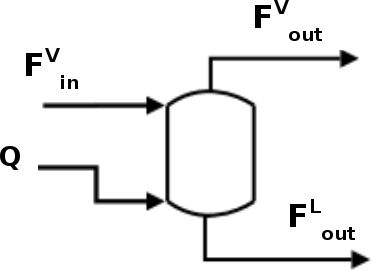
\includegraphics[scale=0.5]{images/Chap3/esquemacondenser2.png}
\caption{Modelo esquemático de um condensador parcial dinâmico.}
\label{fig:condenser}
\end{figure}

O equacionamento básico é mostrado a seguir.

Balanço molar por componente:
\begin{equation}
\dfrac{dM_i}{dt} = F_{in}^V \cdot y_{in_i} - F_{out}^L  \cdot x_{out_i} - F_{out}^V \cdot y_{out_i}  \qquad i=1,2,\cdots,c
\end{equation}
Balanço de energia:
\begin{equation}
\dfrac{dE}{dt} = F_{in}^V \cdot h_{in}^V - F_{out}^L  \cdot h_{out}^L - F_{out}^V \cdot h_{out}^V + Q
\end{equation}
Acúmulos:
\begin{equation}
M_i = M^L \cdot x_{out_i} + M^V \cdot y_{out_i}  \qquad i=1,2,\cdots,c
\end{equation}
\begin{equation}
E = M^L \cdot h_{out}^L + M^V \cdot h_{out}^V - P_{out}^L \cdot V_{cond}
\end{equation}
\nomenclature{$V_{cond}$}{Volume do condensador \nomunit{m^3}}
Restrições das frações molares:
\begin{equation}
\sum_i x_{out_i} = 1
\end{equation}
\begin{equation}
\sum_i x_{out_i} = \sum_i y_{out_i}
\end{equation}
Equilíbrio químico, mecânico e térmico:
\begin{equation}
\hat{\phi}_i^L \cdot x_{out_i} = \hat{\phi}_i^V \cdot y_{out_i}  \qquad i=1,2,\cdots,c
\end{equation}
\begin{equation}
P_{out}^L = P_{out}^V
\end{equation}
\begin{equation}
T_{out}^L = T_{out}^V
\end{equation}
\nomenclature{$T_{out}^L$}{Temperatura de saída da corrente de líquido \nomunit{K}}
\nomenclature{$T_{out}^V$}{Temperatura de saída da corrente de vapor \nomunit{K}}
Restrição geométrica:
\begin{equation}
V_{cond} = M^L \cdot v^L + M^V \cdot v^V
\end{equation}
Nível de líquido:
\begin{equation}
Level = \dfrac {M^L \cdot v^L}{A_{cross}}
\end{equation}

As propriedades físicas e termodinâmicas necessárias são calculadas através de rotinas externas:
\begin{equation}
h_{out}^L = h^L(T_{out}^L, P_{out}^L, x_{out})
\end{equation}
\begin{equation}
h_{out}^V = h^V(T_{out}^V, P_{out}^V, y_{out})
\end{equation}
\begin{equation}
v^L = v^L(T_{out}^L, P_{out}^L, x_{out})
\end{equation}
\begin{equation}
v^V = v^V(T_{out}^V, P_{out}^V, y_{out})
\end{equation}
\begin{equation}
\hat{\phi}_i^L = \hat{\phi}_i^L(T_{out}^L, P_{out}^L, x_{out})  \qquad
i=1,2,\cdots,c
\end{equation}
\begin{equation}
\hat{\phi}_i^V = \hat{\phi}_i^V(T_{out}^V, P_{out}^V, y_{out})  \qquad
i=1,2,\cdots,c
\end{equation}

No \autoref{code:condensadordinamico}, é apresentada a implementação do modelo de condensador dinâmico na linguagem de
modelagem do simulador \emso.
\lstinputlisting[firstline=43, lastline=105, numbers=none, language=EMSO, caption=Modelo de condensador dinâmico. ,
label=code:condensadordinamico] {images/Chap4/condenser.mso}

\subsection{Condensador Estacionário ou Total} \label{sec:modelocondensadorestacionario}
O desenho esquemático de um condensador estacionário pode ser visto na \autoref{fig:condsteady}. O modelo desenvolvido
considera que o equipamento recebe uma corrente totalmente vaporizada e com a retirada de calor, condensa totalmente a
mesma.
\begin{figure}[htb]
\centering 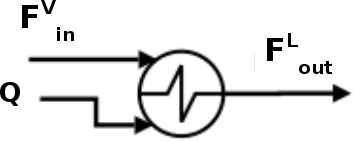
\includegraphics[scale=0.5]{images/Chap3/esquemacondensersteady2.png}
\caption{Modelo esquemático de um condensador estacionário.}
\label{fig:condsteady}
\end{figure}

O modelo é representado pelas seguintes equações:

\begin{flushleft}
Balanço de massa:
\end{flushleft}
\begin{equation}
F_{in}^V = F_{out}^L
\end{equation}
\begin{equation}
y_{in_i} = x_{out_i}  \qquad i=1,2,\cdots,c
\end{equation}
Balanço de energia:
\begin{equation}
F_{in}^V \cdot h_{in}^V + Q = F_{out}^L \cdot h_{out}^L 
\end{equation}
Queda de pressão:
\begin{equation}
\Delta P = P_{in}^V - P_{out}^L
\end{equation}
As propriedades físicas e termodinâmicas necessárias são calculadas através de rotinas externas:
\begin{equation}
h_{out} = h(T_{out}, P_{out}, z_{out})
\end{equation}

O modelo de condensador estacionário, implementado no \emso , pode ser visualizado no
\autoref{code:condensadorestacionario}.
\lstinputlisting[firstline=110, lastline=132, numbers=none, language=EMSO, caption=Modelo de condensador estacionário. ,
label=code:condensadorestacionario] {images/Chap4/condenser.mso}

\section{Prato - Estágio de Equilíbrio} \label{sec:modeloprato}
O modelo de prato representa um estágio de equilíbrio de uma coluna de destilação. Como mostrado no
\autoref{chap:revisaobibliografica}, existem diversas linhas de modelagem de um estágio de equilíbrio.
Dentro da categoria de modelos rigorosos com consideração de equilíbrio termodinâmico entre as fases, o
ponto de maior variação entre os modelos está nas equações relacionadas com a hidrodinâmica do prato,
isto é, nas correlações para o cálculo das vazões internas dos pratos, perfis de pressão e outros
detalhes hidráulicos.
A construção do modelo desenvolvido neste trabalho incluiu a consulta e análise
de inúmeras fontes da literatura, utilizando como base o
trabalho de \citeonline{Gani:1986}.
As correntes envolvidas no modelo são apresentadas no diagrama da
\autoref{fig:prato}:

\begin{figure}[htb]
\centering 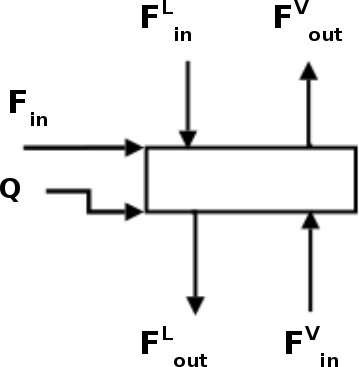
\includegraphics[scale=0.5]{images/Chap3/esquemaprato2.png}
\caption{Modelo esquemático de um prato.}
\label{fig:prato}
\end{figure}

Poderia-se adicionar ainda, uma corrente material de retirada lateral no prato. Com esta corrente ficaria mais fácil
simular colunas que possuem retiradas e refluxos intermediários, comuns na destilação de petróleo. Enquanto esta
corrente adicional não é implementada, deve utilizar um separador de correntes entre pratos de uma coluna e o mesmo
resultado será obtido.

O modelo de prato é composto pelas seguintes equações:
\begin{flushleft}
Balanço molar por componente:
\end{flushleft}
\begin{equation}
\dfrac{dM_i}{dt} = F_{in} \cdot z_{in_i} + F_{in}^L \cdot x_{in_i} + F_{in}^V \cdot y_{in_i} - F_{out}^L  \cdot x_{out_i} -
F_{out}^V \cdot y_{out_i}  \qquad i=1,2,\cdots,c
\end{equation}
Balanço de energia:
\begin{equation}
\dfrac{dE}{dt} = F_{in} \cdot h_{in} + F_{in}^L \cdot h_{in}^L + F_{in}^V \cdot h_{in}^V - F_{out}^L  \cdot h_{out}^L -
F_{out}^V \cdot h_{out}^V + Q
\end{equation}
Acúmulos:
\begin{equation}
M_i = M^L \cdot x_{out_i} + M^V \cdot y_{out_i}  \qquad i=1,2,\cdots,c
\end{equation}
\begin{equation}
E = M^L \cdot h_{out}^L + M^V \cdot h_{out}^V - P_{out}^L \cdot V_{tray}
\end{equation}
\nomenclature{$V_{tray}$}{Volume do prato \nomunit{m^3}}
Restrições das frações molares:
\begin{equation}
\sum_i x_{out_i} = 1
\end{equation}
\begin{equation}
\sum_i x_{out_i} = \sum_i y_{out_i}
\end{equation}
Equilíbrio químico, mecânico e térmico:
\begin{equation}
\hat{\phi}_i^L \cdot x_{out_i} = \hat{\phi}_i^V \cdot y_{eq_i}  \qquad
i=1,2,\cdots,c
\end{equation}
\begin{equation}
P_{out}^L = P_{out}^V
\end{equation}
\begin{equation}
T_{out}^L = T_{out}^V
\end{equation}
Eficiência de Murphree:
\begin{equation}
E_{MV_i} = \dfrac{ y_{out_i} - y_{in_i} } {y_{eq_i} - y_{in_i} } \qquad i=1,2,\cdots,c
\end{equation}
\nomenclature{$E_{MV}$}{Eficiência de prato de Murphree}
Restrição geométrica:
\begin{equation}
V_{tray} = M^L \cdot v^L + M^V \cdot v^V
\end{equation}
Nível de líquido:
\begin{equation}
Level = \dfrac {M^L \cdot v^L}{A_p}
\end{equation}
onde, $A_p$ é a área útil do prato (área do total do prato - área do
\textit{downcomer}), $V_{tray}$ é o volume total do prato, $Level$ é o nível de
líquido e $y_{eq_i}$ é a composição do vapor que está em equilíbrio com o líquido.

\nomenclature{$A_p$}{Área do prato (Área do total do prato -  Área do \textit{downcomer}) \nomunit{m^2}}

Ainda são necessárias duas equações para o cálculo das vazões de líquido e vapor do prato que são função
das propriedades físicas dos fluidos, da geometria do prato, da queda de pressão e do acúmulo de líquido
em cada estágio:
\begin{equation}
F^L = f(M, \textrm{geometria}, \textrm{propriedades fisicas})
\end{equation}
\begin{equation}
F^V = f(\Delta P, \textrm{geometria}, \textrm{propriedades fisicas})
\end{equation}
\nomenclature{$F^L$}{Vazão molar de líquido \nomunit{mol/s}}
\nomenclature{$F^V$}{Vazão molar de vapor \nomunit{mol/s}}

Na \autoref{sec:hydraulics}, é apresentada uma discussão a cerca das
diversas correlações encontradas na literatura para o cálculo da hidrodinâmica do prato.

As propriedades físicas e termodinâmicas necessárias são calculadas através de rotinas externas:
\begin{equation}
h_{out}^L = h^L(T_{out}^L, P_{out}^L, x_{out})
\end{equation}
\begin{equation}
h_{out}^V = h^V(T_{out}^V, P_{out}^V, y_{out})
\end{equation}
\begin{equation}
v^L = v^L(T_{out}^L, P_{out}^L, x_{out})
\end{equation}
\begin{equation}
v^V = v^V(T_{out}^V, P_{out}^V, y_{out})
\end{equation}
\begin{equation}
\rho^L = \rho^L(T_{out}^L, P_{out}^L, x_{out})
\end{equation}
\begin{equation}
\rho^V = \rho^V(T_{out}^V, P_{out}^V, y_{out})
\end{equation}
\begin{equation}
\hat{\phi}_i^L = \hat{\phi}_i^L(T_{out}^L, P_{out}^L, x_{out})  \qquad
i=1,2,\cdots,c
\end{equation}
\begin{equation}
\hat{\phi}_i^V = \hat{\phi}_i^V(T_{out}^V, P_{out}^V, y_{eq}) \qquad
i=1,2,\cdots,c
\end{equation}

O modelo de estágio de equilíbrio foi implementado no simulador \emso\ em etapas. Um modelo básico foi construído com as
equações correspondentes aos balanços e às relações de equilíbrio. O modelo complementar contém as equações da
hidrodinâmica. O \autoref{code:prato} apresenta os modelos.
\lstinputlisting[firstline=38, lastline=154, numbers=none, language=EMSO, caption=Modelos de prato. , label=code:prato]
{images/Chap4/tray.mso}

Com esta divisão, o desenvolvimento de novos modelos de prato fica facilitado. Esta estrutura, baseada no conceito de
herança, ilustrado no \autoref{ap:emso}, permite a reutilização do código presente no modelo básico.
Assim, qualquer modelo novo de estágio de
equilíbrio pode se basear no modelo de prato básico, como o anteriormente apresentado, através da instrução:
\vspace{0.5cm}
\lstinputlisting[firstline=108, lastline=109, numbers=none, caption=Exemplo de modelagem baseada em herança.,
language=EMSO] {images/Chap4/tray.mso}
e conter apenas as novas equações para as vazões internas da coluna.

\section{Colunas de Destilação} \label{sec:modelocolunas}
Com os modelos dos acessórios apresentados anteriormente, várias configurações de colunas podem ser montadas, de acordo
com o equipamento real a ser modelado. Pode ser modelada desde uma simples seção de coluna (Figura
\autoref{fig:secaocoluna}) até uma coluna com condensador e refervedor dinâmicos (Figura \autoref{fig:colunadinamica}).

\begin{figure}[htb]
\centering
  \subfloat[Seção de coluna]{\label{fig:secaocoluna} 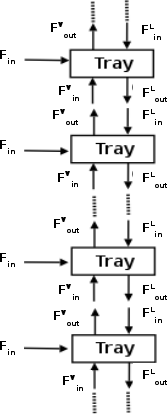
\includegraphics[scale=0.55]{images/Chap3/section2.png}}
  \qquad
  \subfloat[Coluna completa]{\label{fig:colunadinamica} 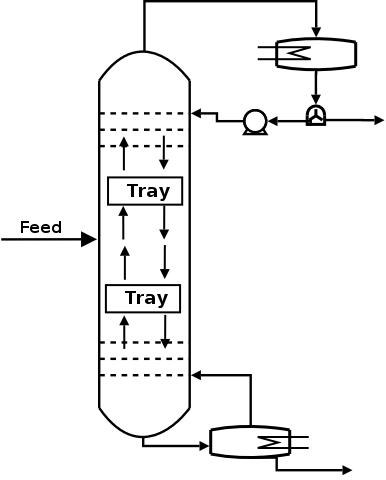
\includegraphics[scale=0.3]{images/Chap3/distKettlecond.png}}
  \caption{Diferentes configurações de colunas de destilação.}
  \label{fig:colunas}
\end{figure}

Para a construção de colunas de destilação com retiradas laterais e refluxos externos, como já mencionado
na \autoref{sec:modeloprato}, deve-se adicionar separadores de correntes entre os pratos, já que o modelo de
estágio de equilíbrio não contém um corrente de saída extra.
O \autoref{code:secao} corresponde à implementação de uma seção de coluna, como a apresentada na Figura
\autoref{fig:secaocoluna}, na linguagem de modelagem do \emso\ . O \autoref{code:colunadinamica} corresponde à
implementação de uma coluna de
destilação como a apresentada na Figura \autoref{fig:colunadinamica}, também
na linguagem do simulador.
\lstinputlisting[firstline=46, lastline=67,
numbers=none, language=EMSO, caption=Modelo de seção de coluna de destilação. , label=code:secao] {images/Chap4/column.mso}

Como pode ser visto na implementação acima, além dos parâmetros necessários para a utilização de cálculos
termodinâmicos externos ($NComp$: número de componentes e $PP$: pacote de propriedades termodinâmicas),
foram declarados alguns parâmetros adicionais: \textit{topdown}, \textit{top} e \textit{bot}.
Estes parâmetros são utilizados para auxiliar nas conexões das correntes internas das colunas. O usuário é responsável
por fornecer o valor de \textit{topdown}, que deve ser 1 se a contagem dos pratos da coluna começa pelo topo
ou -1 se a contagem dos pratos começa pelo fundo. Os parâmetros \textit{top} e \textit{bot} representam
o prato do topo e do fundo da coluna respectivamente. Assim, se $topdown = 1$ o prato do topo é o prato $1$ ($top=1$)
e o prato do fundo o $NTrays$  ($bot = NTrays$). Por outro lado, se $topdown = -1$ o prato do topo
é o prato $NTrays$ ($top=NTrays$) e o prato do fundo o $1$ ($bot = 1$). Esta convenção é necessária para
a realização das conexões entre as vazões dos estágios bem como a visualização dos resultados gerados na simulação.

A conexão entre os $NTrays$ pratos da torre é realizada na seção \textit{CONNECTIONS}. A vazão de vapor que
deixa o prato inferior é conectada à vazão de vapor que entra no prato superior assim como a vazão de líquido
que escoa do prato superior é ligada à vazão de líquido que entra no prato inferior. Com estas conexões, as vazões
internas de uma seção de coluna ficam determinadas e o modelo representado pela Figura \autoref{fig:secaocoluna} é
construído.

\lstinputlisting[firstline=77, lastline=125, numbers=none, language=EMSO, caption=Modelo de coluna de destilação com
condensador e refervedor dinâmicos. , label=code:colunadinamica] {images/Chap4/column.mso}

Vale ressaltar que os modelos de coluna acima apresentados foram construídos com base no conceito de composição
da programação orientada a objetos. Esta característica da linguagem fica evidente quando são declaradas
como variáveis do modelo da coluna outros modelos básicos já existentes, por exemplo:
\lstinputlisting[firstline=91, lastline=97, numbers=none, caption=Exemplo de modelagem baseada em composição.,
language=EMSO] {images/Chap4/column.mso}

Podem ser construídas colunas de destilação de diversas configurações, basta
declarar, na seção de variáveis, diferentes tipos de condensadores,
refervedores e tanques de acúmulo.
Por exemplo, com os modelos básicos apresentados neste capítulo pode-se montar
facilmente uma torre com condensador e refervedor estacionários e tanques no topo e fundo:
\lstinputlisting[firstline=1, lastline=10, numbers=none, caption= Outro exemplo de modelagem baseada em composição.,
language=EMSO] {images/Chap4/composicao.mso}
A diferença entre os modelos está apenas nos tipos de acessórios das colunas e nas conexões entre as correntes internas
da mesma.

No \autoref{code:colunadinamica}, as conexões necessárias, de acordo com a Figura \autoref{fig:colunadinamica}, são:
\begin{itemize}
 \item a conexão da corrente de saída de vapor do refervedor com a entrada de vapor do prato de fundo da coluna;
 \item a conexão da saída de vapor do prato inferior à entrada de vapor do prato superior, ao longo de
todos os pratos da coluna;
 \item a conexão da saída de vapor do prato de topo da columa com a entrada de vapor do condensador;
 \item a conexão da saída de líquido do condensador na entrada de um \textit{splitter};
 \item a conexão de uma das saídas do \textit{splitter} com a entrada da bomba (a outra saída do \textit{splitter} é a
corrente de destilado);
 \item a conexão da saída da bomba com a entrada de líquido do prato do topo da coluna;
 \item a conexão da saída de líquido do prato superior com a entrada de líquido do prato inferior, ao longo de toda
a coluna;
 \item a conexão da saída de líquido do prato do fundo na entrada de líquido de refervedor.
\end{itemize}


\section{Hidráulica de Pratos}\label{sec:hydraulics}
Uma coluna de destilação consiste de um cilindro vertical com diâmetro que pode variar de poucos centímetros
a alguns metros. Da mesma maneira, o número de pratos de uma torre pode variar de poucas unidades  a
várias dezenas.

Uma característica geral do escoamento na bandeja é o fato de que o líquido é impedido de escoar para
o prato abaixo através dos furos pela vazão ascendente de vapor. Assim, enquanto o vapor flui verticalmente
entre os pratos, o líquido escoa horizontalmente na superfície da bandeja caracterizando o fluxo cruzado.
Os três principais tipos de pratos encontrados em unidades industriais são:
pratos perfurados, valvulados, e pratos com borbulhadores. Na
\autoref{fig:traytypes} são mostradas as diferentes aberturas encontradas nesses pratos e o caminho a ser realizado pelo vapor para atravessá-lo.
\begin{figure}[htb]
\centering 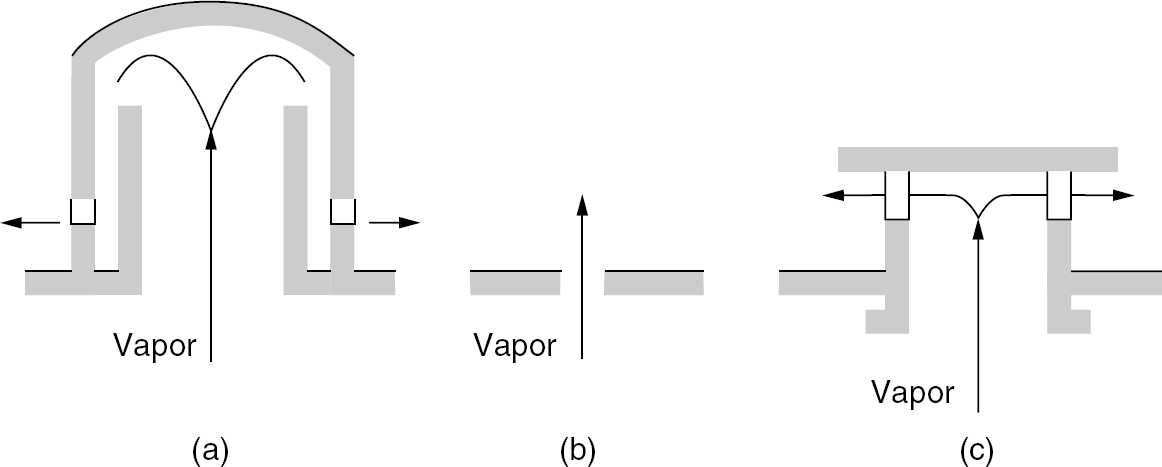
\includegraphics[scale=0.5]{images/Chap3/traytype.png}
\caption{Diferentes tipos de aberturas dos pratos: (a) borbulhadores, (b)
furo e (c) válvula.}
\label{fig:traytypes}
\end{figure}

Apesar das diferentes configurações de colunas de destilação de pratos, todas possuem
características em comum que permitem que as mesmas sejam descritas de uma maneira generalizada através
de uma modelagem mais simplificada. Estas generalizações são importantes para o estudo do comportamento
hidráulico do prato mesmo em se tratando de um tipo específico de bandeja. Isto deve-se ao fato da alta
complexidade de análise do fluxo cruzado que acontece entre o líquido e o vapor. Sendo assim,
sempre são feitas algumas considerações simplicativas na elaboração de correlações de queda de pressão
e vazão de líquido \cite{Khoury:2005}.

Os principais fatores que influenciam o desempenho do prato são: a formação de espuma, o arraste de líquido e vapor,
o gradiente na concentração de líquido no prato, gotejamento, inundação e a queda de pressão.
Quando é realizado o projeto de uma coluna de destilação todos estes fatores são considerados pois a maioria
deles é conseqüência da capacidade da coluna e das vazões internas de líquido e vapor que caracterizam o ponto
de operação a que a mesma será submetida.
Diversos níveis de modelagem podem ser realizados considerando todos ou parte destes fatores citados.
Modelos rigorosos com simplificações na hidráulica levam em conta
apenas a formação de bolhas, que afeta diretamente a quantidade de líquido no prato e conseqüentemente
o seu grau de aeração, e a queda de pressão do equipamento.

Nas próximas seções serão apresentadas as principais correlações de hidrodinâmica encontradas na literatura e uma
discussão sobre as mesmas.

\subsection{Vazão de vapor - Queda de Pressão}\label{sec:vapflow}
A força motriz para o escoamento do líquido em uma torre é a força da gravidade. Já para o escoamento de vapor acontecer
deve existir uma diferença de pressão ao longo da coluna. Assim, os pratos inferiores devem ser mantidos em uma
pressão superior aos do topo. Além disso, um gradiente mínimo de pressão é
necessário para evitar gotejamento de líquido através das aberturas dos pratos \cite{Khoury:2005}.

Segundo \citeonline{Lockett:1986} a queda de pressão em um estágio, $h_{WT}$, é a soma de três contribuições,
aqui representadas em termos da altura de líquido (\textit{head}):
\begin{equation}
h_{WT} = h_{DT}+h_{cl}+h_R
\end{equation}
onde $h_{DT}$ representa a queda de pressão do prato seco, isto é, a resistência ao escoamento do vapor mesmo quando
não há líquido no prato; $h_{cl}$ é a queda de pressão devido ao acúmulo de líquido claro e $h_R$ é uma queda de pressão
residual referente à tensão superficial dos fluidos.

Ainda segundo \citeauthoronline{Lockett:1986}, a queda de pressão do prato seco pode ser calculada por:
\begin{equation}
h_{DT} = \dfrac{\xi \rho_{vap} u^2_ h}{2 g \rho_{liq}}
\end{equation}
onde $u_ h$ é a velocidade do vapor através dos furos do prato e $\xi$ é o chamado coeficiente de orifício,
que é uma função principalmente do número de Reynolds do orifício $Re_h$
e de parâmetros geométricos do prato. Para uma visão mais detalhada sobre correlações para o cálculo de $\xi$ e $h_{DT}$,
ver \citeonline{Lockett:1986}.
\nomenclature{$g$}{Aceleração da gravidade\nomunit{m/s^2}}
A contribuição da altura de líquido para a queda de pressão pode ser calculada por:
\begin{equation}
h_{cl} = \dfrac{\left( P_1 - P_2\right) + u_S \rho^V \left(u_h - u_S \right) }{g \rho^L}
\end{equation}
onde $P_1$ é a pressão no fundo do prato, $P_2$ é a pressão acima do líquido,
$u_ S$ é a velocidade superficial do vapor e $g$ é a aceleração da gravidade.

Existem diversas correlações para a queda de pressão residual. Os fatores mais relevantes na sua determinação
são as propriedades físicas dos fluidos e a razão espessura do prato/diâmetro do furo. Devido à sua pequena
contribuição, para pratos valvulados este termo pode ser ignorado sem maiores problemas. Já para pratos perfurados
pode ser calculada de uma forma simplificada por:
\begin{equation}
h_{R} = \dfrac{4\sigma }{d_h \rho^L g}
\end{equation}
onde $\sigma$ corresponde à tensão superficial do líquido e $d_h$ ao diâmetro do furo.

Apesar de todo o rigorismo proposto para o cálculo da queda de pressão do prato, geralmente são utilizadas correlações
mais simplificadas na construção de modelos. A contribuição da tensão superficial é geralmente ignorada e
a queda de pressão
do prato seco se resume a um parâmetro. A pressão devido ao acúmulo de líquido é calculada através da fórmula
convencional de pressão hidrostática. Sendo assim, o $\Delta P$ se resume a uma equação que é função da altura
de líquido no prato, da vazão de vapor e de propriedades físicas do fluido. Na \autoref{tab:flowvapcorrelations},
as principais correlações encontradas na literatura são mostradas.
\begin{table}[p]
\caption{Correlações para cálculo da queda de pressão em função da vazão de vapor.}
\label{tab:flowvapcorrelations}
\begin{center}
\begin{tabular}{lp{0.7\textwidth}} % {lp{0.5\textwidth}cc}
\hline
\textbf{Fonte} &  \hspace{0.2\textwidth}\textbf{Correlação} \\ \hline
\citeonline{Feehery:1998} &
\begin{equation}
\label{eq:feehery}
\begin{array}{l}
\Delta P = \Delta P^{static} + \Delta P^{dry} \\
\Delta P^{static} = \dfrac{V_{liq}}{A_p} \cdot \rho_{vap} \cdot g\\
\Delta P^{dry} = \rho^V \left( \dfrac{F^V \cdot Mw}{\rho^V} \cdot A_{a} \cdot w\right) ^2\\
\end{array}
\end{equation}
 \\
\hline
\citeonline{Roffel:2000} &
\begin{equation}
\begin{array}{l}
\Delta P = \Delta P^{dry} + \beta \dfrac{M \cdot Mw}{A_{cross}} \cdot g \cdot 10^5 \\
\Delta P^{dry} = 0,0013 \left( \dfrac{F^V \cdot Mw}{\rho^V \cdot A_{h}}\right) ^{1,08}\\
% \cdot bar \left(\dfrac{s}{m}\right)^{1.08} \cdot
\Delta P=bar, F^V=kmol/s, Mw=kg/kmol \\ \rho^V=kg/m^3,  A_{h}=m^2
\end{array}
\end{equation}
 \\
\hline
\citeonline{Klingberg:2000} &
\begin{equation}
\begin{array}{l}
\Delta P = \Delta P_{tr} +g \cdot \rho^L \cdot Level \\
\Delta P_{tr} = f(F_{S})\\
F_{S} = u_S \cdot \rho^{V\ 0,5} \\
u_S \cdot \rho^V \cdot A_{cross} = Mw_V \cdot F^V
\end{array}
\end{equation}
 \\
\hline
\citeonline{Reepmeyer:2003} &
\begin{equation}
\begin{array}{l}
\Delta P = \left( \dfrac{F^V \cdot v^V}{A_h}\right)^2 \cdot \dfrac{\rho^V \cdot c_w}{2} \\
\end{array}
\end{equation}
 \\
\hline
\citeonline{Wang:2003} &
\begin{equation}
\begin{array}{l}
\Delta P = \left(  \dfrac{F^V \cdot v^V}{A}\right)^2 \cdot \rho^V \cdot \alpha +  \rho^L \cdot g \cdot Level\\
\end{array}
\end{equation}
 \\
\hline
\citeonline{Elgue:2004} &
\begin{equation}
\begin{array}{l}
\Delta P = m\Delta P\\
m\Delta P = cte\ ou\\
m\Delta P = \beta^{tray} \cdot F^{V\ 2}\\
\end{array}
\end{equation}
 \\
\hline
\citeonline{Ltd.:2004} &
\begin{equation}
\begin{array}{l}
\Delta P = \left(  \dfrac{F^V}{A_h}\right)^2 \cdot \dfrac{\alpha}{\rho^V} + \beta \cdot \rho^L \cdot g \cdot Level\\
\end{array}
\end{equation}
 \\
\hline
\end{tabular}
\end{center}
\end{table}
\nomenclature{$w$}{Constante dependente da geometria do prato presente na \autoref{eq:feehery}}
Um fator importante na escolha de uma correlação para este tipo de cálculo é a análise da consistência de unidades
de medida. Na equação de \citeonline{Roffel:2000}, por exemplo, não se consegue chegar à unidade de pressão em
$\Delta P^{dry}$ sem que seja atribuída uma unidade à constante $0,0013$.

Outra consideração importante na análise das correlações é o seu grau de rigorismo. Se comparadas ao método
de cálculo de \citeonline{Lockett:1986}, as equações apresentadas são todas
simplificadas. Mesmo assim, pode-se dividir estas equações em dois subconjuntos:
as que consideram apenas a contribuição da vazão de vapor e da queda de pressão do prato seco e as que consideram adicionalmente a queda de pressão estática da coluna
de líquido do prato.

Neste trabalho as correlações de \citeonline{Reepmeyer:2003} e \citeonline{Wang:2003} foram implementadas e
comparadas. Para a comparação foram utilizados dados reais de operação de uma coluna deisobutanizadora,
comparando-se os perfis de temperatura e pressão ao longo da coluna.
A equação de \citeonline{Reepmeyer:2003} apresentou melhores resultados mas não mostrou muita
robustez em algumas simulações. Pois, pequenas variações no parâmetro $c_w$, envolvido nesta correlação,
são capazes de gerar grandes impactos na resposta do modelo. Além disso, esta correlação
apresentou uma maior freqüência de falhas numéricas nos testes realizados.
Por outro lado, a equação de \citeonline{Wang:2003} se apresentou mais estável por contar com a contribuição da pressão estática à pressão total. O termo ($\rho^L \cdot g \cdot Level$)
confere à correlação um amortecimento às variações da vazão de vapor, que são muito grandes
quando se trata de um procedimento de partida de uma coluna.
Porém, como a primeira correlação apresentou melhores resultados na comparação entre dados experimentais \textit{versus}
modelo, esta foi a escolhida neste estudo.

Outra consideração importante é que a equação explícita em $\Delta P$
deixa o sistema de equações mais propenso a falhas de integração do que a correlação explícita em $F$.
Finalmente, após a análise das equações apresentadas, a forma final da equação que é utilizada neste estudo é:
\begin{equation}
\label{eq:vapfinal}
F^V = \dfrac{A_h}{v^V} \cdot \sqrt{\dfrac{\left( P_{in}^V - P_{out}^V\right)}{\rho^V \cdot \alpha}}
\end{equation}
onde, $A_h$ é a área total dos furos do prato e $\alpha$ é o coeficiente de
queda de pressão no prato seco, utilizado como parâmetro de ajuste.

\nomenclature{$h_{cl}$}{Altura de líquido claro no prato \nomunit{m}}
\nomenclature{$u_h$}{Velocidade do vapor através dos furos do prato \nomunit{m/s}}
\nomenclature{$u_S$}{Velocidade superficial do vapor: ($\frac{Q_h}{A_a}$) \nomunit{m/s}}
\nomenclature{$Q_h$}{Vazão volumétrica de vapor através dos furos do prato \nomunit{m^3/s}}
\nomenclature[G]{$\xi$}{Coeficiente de orifício}
\nomenclature{$c_w$}{Resistência ao escoamento de vapor}
\nomenclature[G]{$\sigma$}{Tensão superficial \nomunit{N/m}}
\nomenclature{$d_h$}{Diâmetro do furo \nomunit{m}}
\nomenclature[G]{$\beta^{tray}$}{Constante relacionada com propriedades físicas do prato}
\nomenclature[G]{$m\Delta P$}{Modelo para o cálculo da queda de pressão \nomunit{Pa}}
\nomenclature{$F_S$}{Fator superficial \nomunit{kg^{0.5}/m^{0.5}/s}}
\nomenclature{$A_h$}{Área total dos furos do prato \nomunit{m^2}}
\nomenclature{$P_{out}^V$}{Pressão da corrente de vapor que sai do equipamento \nomunit{atm}}
\nomenclature{$P_{out}^L$}{Pressão da corrente de líquido que sai do equipamento \nomunit{atm}}
\nomenclature{$P_{in}^V$}{Pressão da corrente de vapor que entra no equipamento \nomunit{atm}}
\nomenclature{$P_{in}^L$}{Pressão da corrente de líquido que entra no equipamento \nomunit{atm}}
\nomenclature[G]{$\alpha$}{Coeficiente de queda de pressão no prato seco}
\nomenclature[G]{$\Delta P$}{Diferença de pressão \nomunit{atm}}

\subsection{Vazão de líquido}\label{sec:liqflow}
A predição do acúmulo de líquido em cada prato e também do seu escoamento através do vertedouro é muito importante
na previsão do comportamento hidráulico de uma coluna de destilação. A altura de líquido exerce influência na
queda de pressão, eficiência do prato, nos limites de operação da coluna e no regime de escoamento do estágio.
O cálculo
da altura de líquido depende das propriedades da mistura e de parâmetros
geométricos tais como a altura e comprimento do vertedouro, a área de furos do prato, o diâmetro dos furos e outros.
As correlações existentes para a predição da altura de líquido são todas empíricas e, segundo \citeonline{Wijn:1999},
não são consideradas satisfatórias.

Existem vários trabalhos na literatura descrevendo a relação entre a altura de líquido, a quantidade
de vapor disperso na fase líquida e a sua vazão. Os métodos mais antigos expressam a altura de líquido como uma
função linear da altura do vertedouro e dos acúmulos de líquido e vapor. Nesta linha, outros
trabalhos evoluíram
da relação linear para uma função exponencial envolvendo também alguns parâmetros geométricos do prato. Depois, a altura
de líquido passou a ser considerada como a contribuição de duas parcelas, uma abaixo e outra acima do vertedouro
\cite{Wijn:1999}.

Dependendo do regime de operação da coluna (regime de \textit{spray} ou regime de bolhas, por exemplo),
o transporte
do líquido para o prato inferior pode acontecer de várias maneiras além do simples escoamento do líquido através
do vertedouro. Assim, a complexidade na modelagem desse transporte pode variar de uma relação clássica baseada na
equação de Francis (\autoref{eq:francis}) até a previsão de respingos de líquido
ocasionados pelo rompimento de bolhas em um regime de \textit{spray}.
% \begin{equation}
% F_{outL} \cdot Mw = \rho_{liq}  \cdot lw \cdot \left( \dfrac{h_{ow}}{750}\right)^{1,08}
% \end{equation}
% com $F_{outL}$ em $kmol/h$, $Mw$ em $kg/kmol$, $\rho_{liq}$ em $kg/m^3$, $lw$ em $m$ e $h_{ow}$ em $mm$.

No trabalho de \citeonline{Klingberg:2000}, a altura de líquido, $Level$, é calculada pela contribuição da
altura do vertedouro, $h_w$, e da altura da dispersão de líquido e vapor acima do mesmo, $h_{ow}$, sendo relacionada
com a vazão através da expressão:
\begin{equation}
h_{ow} = \dfrac{1,45}{g^{\frac{1}{3}}} \left( \dfrac{\frac{F_{out}^L}{lw}}{\varepsilon_l}\right)^{\frac{2}{3}} + \dfrac{c}{2g\left( \rho^V - \rho^L \right)} \left( \dfrac{F_S - 0,2\sqrt{\rho^V}} {1 - \varepsilon_l} \right)^2 
\end{equation}
onde $\varepsilon_l$ é a fração de líquido na espuma e $c$ é uma constante adimensional.
\nomenclature[G]{$\varepsilon_l$}{Fração de líquido na espuma}
\nomenclature[G]{$\varepsilon_w$}{Fração de vapor na espuma que escoa sobre o vertedouro}

Em \citeonline{Lockett:1986}, a mesma relação é utilizada, $Level = h_w + h_{ow}$. O nível total é uma função linear
do fator superficial, $F_S$, dos parâmetros geométricos ($h_w$, $lw$) e da
vazão volumétrica de líquido, $Q^L$:
\begin{equation}
Level = A h_w + B F_S + C \dfrac{Q^L}{lw} + D
\end{equation}
com os parâmetros $A,\ B,\ C,\ e\ D$ variando conforme o tipo de prato e mistura a ser destilada. Vários conjuntos
de valores podem ser encontrados em \citeonline{Lockett:1986}.
A altura de espuma acima do vertedouro é dada pela equação de Francis:
\begin{equation}
\label{eq:francis}
h_{ow} = \dfrac{1,04}{C_d^{0,67} g^{0,33}} \left(
\dfrac{Q^L}{\left(1-\varepsilon_w \right) lw } \right)^{0,67}
\end{equation}
onde $C_d$ é o coeficiente de descarga, $g$ é a aceleração da gravidade em
$m/s^2$, $Q^L$ é a vazão volumétrica de líquido em $m^3/s$, $lw$ o comprimento do vertedouro em $m$ e $\varepsilon_w$ é a fração de vapor na espuma que escoa sobre o
vertedouro.

Além das duas formulações mostradas anteriormente, muitas outras equações são apresentadas na literatura para o
cálculo da vazão de líquido em uma coluna de destilação. A grande maioria delas é baseada na clássica equação de
Francis, que trata de uma relação simples entre a altura de líquido e a vazão. As principais correlações
encontradas estão listadas na \autoref{tab:liqflowcorrelations}.

\begin{table}[p]
\caption{Correlações para cálculo da vazão de líquido em colunas de destilação.}
\label{tab:liqflowcorrelations}
\begin{center}
\begin{tabular}{lp{0.7\textwidth}} % {lp{0.5\textwidth}cc}
\hline
\textbf{Fonte} &  \hspace{0.2\textwidth}\textbf{Correlação} \\ \hline
\citeonline{Olsen:1997} &
\begin{equation}
\begin{array}{l}
F^L = \dfrac{lw N_p \rho^L}{Mw \left( 0,665 F_W\right)^{\frac{3}{2}} } \left( \dfrac{M^L Mw}{\rho^L A_a} - h_w \right)^{\frac{3}{2}} - P_l
\end{array}
\end{equation}
 \\
\hline
\citeonline{Feehery:1998} &
\begin{equation}
\begin{array}{l}
% F_{outL} = \dfrac{lw \rho_{liq}}{Mw} \left( \dfrac{\frac{V_{liq}}{A_p} - h_w} {750}\right)^{\frac{3}{2}}
F^L = \dfrac{lw \rho^L}{Mw} \left( \dfrac{h_{ow}} {750}\right)^{\frac{3}{2}}
\end{array}
\end{equation}
 \\
\hline
\citeonline{Roffel:2000} &
\begin{equation}
\label{eq:roffel}
\begin{array}{l}
F^L = \dfrac{2}{3} \sqrt{2g} \dfrac{\rho^L}{Mw} lw\ \phi\ h_{ow}^{\frac{3}{2}}\\
\phi = 2\beta-1 \\
\beta = 1- 0,3593 \left(\dfrac{F^V Mw} {A_{cross} \sqrt{\rho^V}} \right)^{0,177709} \\
h_{ow} = \dfrac{M^L Mw}{A_{cross} \rho^L \phi}
\end{array}
\end{equation}
 \\
\hline
\citeonline{Wang:2003} &
\begin{equation}
\label{eq:wang}
\begin{array}{l}
F^L = \alpha_w \ lw \dfrac{\left(\frac{Level - \beta h_w}{\beta} \right)^{\frac{3}{2}} }{v^L}\\
\end{array}
\end{equation}
 \\
\hline
\citeonline{Reepmeyer:2003} &
\begin{equation}
\begin{array}{l}
F^L = 1,84 \dfrac{lw}{\rho^L} \left( \dfrac{Level - h_w}{cf_w}\right)^{\frac{3}{2}} \\
\end{array}
\end{equation}
 \\
\hline
\citeonline{Ltd.:2004} &
\begin{equation}
\begin{array}{l}
F^L = 1,84 \ \rho^L \ lw \left( Level - h_w\right)^{\frac{3}{2}}
\end{array}
\end{equation}
 \\
\hline
\citeonline{Osorio:2004} &
\begin{equation}
\label{eq:osorio}
\begin{array}{l}
F^L = k_w \ d_w \ lw \left( Level - h_w\right)^{\frac{3}{2}}
\end{array}
\end{equation}
 \\
\hline
\end{tabular}
\end{center}
\end{table}
\nomenclature[G]{$\phi$}{Densidade relativa da espuma, \autoref{eq:roffel}}
\nomenclature[G]{$\alpha_w$}{Coeficiente da equação \autoref{eq:wang}, \nomunit{m^{0,5}/s}}
\nomenclature{$k_w$}{Coeficiente da \autoref{eq:osorio}, \nomunit{mol/(s\ cm^{\frac{5}{2}})}}
Na correlação de \citeonline{Olsen:1997}, $F^L$ é em $kmol/s$, $lw$ em $m$, $\rho^L$ em $kg/m^3$, $Mw$ em $kg/kmol$,
$M^L$ em $kmol$, $A_a$ em $m^2$, $h_w$ em $m$ e $P_l$ em $koml/s$. Na correlação de \citeonline{Feehery:1998}, as
unidades são: $F^L$ em $kmol/h$, $Mw$ em $kg/kmol$, $\rho^L$ em $kg/m^3$, $lw$ em $m$ e $h_{ow}$ em $mm$.
Na equação apresentada por \citeonline{Roffel:2000}, $F^L$ e $F^V$ são em $kmol/s$, $g$ é a aceleração da
gravidade em $m/s^2$, $\rho^L$ e $\rho^V$ são em $kg/m^3$, $Mw$ em $kg/kmol$, $lw$ e $h_{ow}$ em $m$,
$A_{cross}$ em $m^2$ e $M^L$ em $kmol$. Na equação de \citeonline{Wang:2003} e \citeonline{Reepmeyer:2003},
$F^L$ é expresso em $mol/s$, $lw$, $Level$ e $h_w$ em $m$, $v^L$ em $m^3/mol$ e $\rho^L$ em $kg/m^3$.
Na correlação apresentada em \citeonline{Ltd.:2004}, a equação está em base mássica com $F^L$ em $kg/s$,
$\rho^L$ em $kg/m^3$ e $lw$, $Level$ e $h_w$ em $m$. Por fim, na equação de \citeonline{Osorio:2004}, as
unidades são: $F^L$ em $mol/s$, $k_w$ em $mol/s\ cm^{\frac{5}{2}}$ e $d_w$, $lw$, $Level$ e $h_w$
em $cm$.

O grande problema das equações para o cálculo da vazão de líquido está na determinação de seus parâmetros. Quando um
modelo é construído para representar uma unidade já existente, estes parâmetros
são utilizados como parâmetros de ajuste da resposta
simulada aos dados reais de operação. Mas, quando se quer utilizar o modelo
para o projeto de um processo novo, a falta destas informações acaba inviabilizando o seu uso.
Como pode ser visto na \autoref{tab:liqflowcorrelations},
a equação de \citeonline{Roffel:2000} é a única que relaciona todas as variáveis importantes no comportamento
do líquido no prato para o cálculo da sua vazão sem envolver parâmetros
empíricos adicionais.
Porém,
% esta correlação deve ser utilizada com muito
% cuidado uma vez que envolve constantes que não são adimensionais, como o
% número $0,3593$. Neste caso,
% a utlização fica limitada às unidades de medida
% utilizadas no desenvolvimento da correlação. Além disso,
a utilização em
equipamentos com uma geometria diferente do equipamento original (utilizado na
determinação das constantes da correlação) fica comprometida.
% A equação utilizada neste trabalho foi baseada na estrutura da correlação apresentada por
% \citeonline{Wang:2003} e nos parâmetros
% da equação de \citeonline{Reepmeyer:2003}. A forma final da correlação utilizada é:
% \begin{equation}
% F_{outL} = 1,84 \ lw \dfrac{\left(\frac{Level - \beta h_w}{\beta} \right)^{\frac{3}{2}} }{v_{liq}}\\
% \end{equation}

Pelos motivos acima citados e pelo desempenho nas simulações do processo
apresentado no \autoref{chap:coldeiso}, a equação utilizada neste trabalho foi
a apresentada por \citeonline{Wang:2003}:
\begin{equation}
F^L = \alpha_w \ lw \dfrac{\left(\frac{Level - \beta h_w}{\beta} \right)^{\frac{3}{2}} }{v^L}\\
\end{equation}
onde, $\alpha_w$ e $\beta$ são parâmetros de ajuste do modelo.

\nomenclature{$cf_w$}{Resistência ao escoamento de líquido}
\nomenclature{$d_w$}{Diâmetro do vertedouro \nomunit{cm}}
\nomenclature{$V_{liq}$}{Volume de líquido no prato \nomunit{m^3}}
\nomenclature{$A_a$}{Área ativa do prato \nomunit{m^2}}
\nomenclature{$P_l$}{Vazão de produto \nomunit{kmol/s}}
\nomenclature{$Mw$}{Massa molar média da mistura\nomunit{g/mol}}
\nomenclature{$F_W$}{Correção da altura do vertedouro}
\nomenclature{$N_p$}{Número de passes}
\nomenclature{$lw$}{Comprimento do vertedouro \nomunit{m}}
\nomenclature[G]{$\beta$}{Coeficiente de aeração}
\nomenclature{$h_w$}{Altura do vertedouro \nomunit{m}}
\nomenclature{$h_{ow}$}{Altura de líquido acima do vertedouro \nomunit{m}}
\nomenclature{$Q^L$}{Vazão de líquido \nomunit{m^3/s}}
\nomenclature[G]{$\varepsilon$}{Fração de vapor na espuma}
\nomenclature{$C_d$}{Coeficiente de descarga}
% \nomenclature{$\Upsilon$}{Constante da equação de \citeonline{Wang:2003} ($m^{0,5} / s$)}

%\include{Chap4}
%\include{Chap5}
%\include{Chap6}
%
% 
%
\chapter{Conclusões} \label{chap:conclusoes}
% 
% Como se sabe, a operação de colunas de destilação vem sendo estudada há muitos anos.
% Sabe-se também, que este
% equipamento é um dos mais importantes das indústrias químicas, petroquímicas e de alimentos. Sua
% importância não se resume só a sua função e operação, mas também devido ao fato de que
% colunas de destilação são responsáveis por grande parte do gasto de energia em uma
% indústria. Sendo assim, o desenvolvimento de modelos para estes equipamentos é uma tarefa
% relevante, tanto para projeto quanto para simulações de operação e otimização das
% unidades existentes.

Modelos matemáticos de colunas de destilação podem ser classificados de acordo com o seu
grau de detalhamento: se possuem predição da composição, temperatura e vazões para cada prato,
os chamados modelos rigorosos, ou se são compostos por uma descrição global da coluna
utilizando um menor número de variáveis, baseados em algum tipo de interpolação, os modelos
reduzidos. Neste trabalho, foram apresentadas as diversas formas de
modelagem de sistemas de separação e concluiu-se que a escolha das considerações
simplificativas varia com a aplicação do modelo. Em estudos onde são necessárias simulações
repetitivas, como em otimizações, os modelos reduzidos podem ser os indicados.
Mas, em estudos de partidas e paradas de colunas de destilação é importante que o
comportamento dinâmico do sistema seja bem representado levando ao uso de
modelos rigorosos completos. 

Na linha da modelagem baseada no equilíbrio termodinâmico entre as fases líquida e vapor, foram
desenvolvidos todos os modelos necessários para a confecção de um modelo genérico de coluna
de destilação. Os modelos foram implementados no simulador dinâmico de processos EMSO
utilizando seu ambiente de modelagem e sua linguagem própria. Os modelos gerados neste estudo
fazem parte da biblioteca EML (EMSO Model Library). Esta biblioteca é distribuída no conceito
de \emph{software} livre, disponibilizando todos os modelos via internet e sem
custo.

Um exemplo de uma coluna de destilação reativa serviu como ilustração para a aplicação
dos modelos desenvolvidos neste trabalho em partidas de unidades de separação.
Ao contrário da modelagem encontrada na literatura para esse tipo de sistema, a condição de
equilíbrio termodinâmico entre as fases líquida e vapor foi considerada desde o início da
simulação sem causar problemas de inicialização e integração, conforme alguns autores relatam.
A partida de uma
coluna vazia e fria foi simulada de acordo com três das estratégias convencionais encontradas
na literatura. Como esperado, a partida realizada com refluxo total para a coluna apresentou um
tempo de transientes maior que as demais. Além disso, o modelo apresentado se mostrou muito
indicado para simulações de partida, uma vez que possíveis dificuldades para a determinação de
seus principais parâmetros não afetam a análise do tempo de operação dinâmica.

Outro exemplo foi utilizado para a validação do modelo desenvolvido. Trata-se de uma coluna
deisobutanizadora da PETROBRAS composta de 80 pratos que separa isobutano de
uma mistura de 13 componentes. Algumas pequenas adaptações foram realizadas nos modelos e os resultados obtidos
foram satisfatórios. Tanto a resposta estacionária quanto o comportamento dinâmico da
unidade foram comparados. O problema gerou um sistema de mais de 6300 equações. Um período de
8 dias de operação com várias perturbações na carga e no refluxo da coluna foi simulado em
cerca de 19 minutos de CPU. Conclui-se com isto que este modelo pode ser aplicado para os
mais diversos fins, desde simulações de procedimentos de parada e partidas de unidades, até
estimações, otimizações e treinamento de operação.

Como perspectivas de trabalhos futuros, algumas melhorias podem ser feitas nos modelos apresentados.
Para tornar o modelo de prato ainda mais genérico, pode ser adicionada uma corrente material extra
correspondente a uma retirada lateral. Isto permitiria a modelagem de colunas de destilação de petróleo
sem utilizar separadores de correntes entre os estágios da coluna.
A modelagem fiel do controle de pressão do topo da torre através do \textit{hot bypass} também é um assunto
interessante a ser estudado. Provavelmente esta implementação melhoraria a capacidade de predição do modelo
principalmente nas condições do topo da coluna.
Além disso, alguns assuntos importantes sobre a modelagem
de sistemas de separação podem ser estudados.
Sabe-se que na indústria, grande parte das colunas de destilação operam muito próximo
do seu limite superior de capacidade. Assim, a previsão do fenômeno de inundação da torre
e suas conseqüências na eficiência de separação se torna muito interessante.
Além de colunas de destilação de pratos, as colunas recheadas também são muito utilizadas.
A adaptação dos modelos apresentados nesta dissertação para a
representação deste tipo de colunas deverá ser a continuidade deste trabalho.



% Comandos para as referencias bibliográficas
\newdimen\bibindent
\setlength\bibindent{1.5em} % identaçao das referencias
{ % Um lineskip menor neste contexto de referencias
\baselineskip 4.3mm
% Edite o arquivo ppgeq.bib com as suas próprias referências
\bibliography{ppgeq}
}

% Inclusao dos Appendices
\appendix
%
%
%
\chapter{Normas do padrão de dissertação/tese/qualify} \label{chap:normas}


\emph{Neste capítulo estão sumarizadas as normas para o padrão de dissertação/tese/qualify
do Programa de Pós-Graduação em Engenharia Química da Universidade Federal do Rio Grande
do Sul (PPGEQ--UFRGS).
O presente documento está de acorodo com estas normas e pode ser utilizado como guia.
Nas seções abaixo são explicitados os padrões assumidos.}

\section{Dimensões e formato geral}

O documento deverá utilizar dimensões padrão A4.
As margens laterais serão de acordo com ABNT, com 3~cm na esquerda e 2~cm direita.
Isto fará com que o documento, após encadernação, fique com 2~cm de margem em
ambos os lados.
O documento deverá ser produzido para a impressão frente e verso.

Ainda de acordo com a ABNT, as margens superior e inferior seriam de 3 e 2~cm, respectivamente.
Entretanto, isto significa em uma perda considerável de espaço, além de uma assimetria.
Fica determinado que as margens superior e inferior serão de 2~cm.

\section{Espaçamento entre linhas e tamanho de fonte}

Seguindo recomendações tipográficas, o tamanho da fonte deve ser tal que o número de caracteres
por linha varie entre 60 e 70. Isto é obtido usualmente com uma fonte tamanho 12.
O espaçamento entre linhas deverá ser de 1,5 no corpo do texto.
Especialmente na seção de referências bibliográficas, o espaçamento será simples.
O corpo do texto deve ser em fonte tipo Times ou similar.

\section{Numeração}

Todo o início de seção (Listagem, Capítulo, Apêndice, etc.) deverá iniciar em página impar,
fazendo com que fique sempre na página à direita do leitor.
Poderá haver necessidade de deixar uma página em branco para respeitar esta regra.
No padrão em \LaTeX{} este comportamento é automatizado. 

As folhas de rosto, listagens, agradecimentos, etc. são numeradas em números romanos
centralizados no rodapé. Estas páginas não contém cabeçalho e devem
conter exatamente as páginas exemplificadas no início deste documento.

A contagem de páginas do documento (com números arábicos) inicia-se na primeira página do Capítulo~1.

A primeira página de cada capítulo não deverá conter cabeçalho, apenas o número da página
centralizada no rodapé.
A páginas do corpo do documento deverão conter um cabeçalho.
Páginas pares deverão apresentar o número da página no extremo esquerdo e a referência ao
capítulo atual no extremo direito.
As páginas ímpares deverão apresentar a referência à seção no extremo esquerdo e o número
da página no extremo direito.

Cada capítulo deverá iniciar com ``Capítulo X'' e, uma linha abaixo, deverá
ser apresentado o título do capítulo.
Também poderá estar presente uma pequena sinopse
em itálico, antes da primeira seção do capítulo.
As seções deverão ser numerádas até 3 níveis. Por exemplo 1.1, 1.2, 1.2.3.
Um quarto nível deverá ser evitado.
Se necessário um quarto nível, este não deverá ser numerado.

Os títulos das seções e capítulos deverão ser em fonte tipo Arial e negrito.
Para o segundo nível de numeração (p. ex. 3.1) deverá ser utilizanda uma fonte maior, tamanho 14.
Para o terceiro nível de numeração (p. ex. 3.2.2) dererá ser utilizado apenas o negrito e
fonte tamanho nornal.
Os textos nos cabeçalhos também em fonte tipo Arial.

O sumário deverá apresentar todas as seções do documento, iniciando com as páginas
das listagens de figuras, tabelas, etc.
O sumário deverá apresentar até o terceiro nível de numeração, ex. 1.2.3.
No sumário, os títulos de capítulos devem estar em fonte tipo Arial e em negrito,
os demais em fonte simples tipo Times.

\section{Ficha catalográfica}

Uma ficha catalográfica deverá estar presente no verso da primeira página do
documento (não no verso da capa -- o que equivale a terceira página do
presente documento).

Verificar se a ficha catalográfica está exatamente como a produzida
pelo sistema disponível em \url{http://sabi.ufrgs.br/servicos/publicoBC/ficha.php}.
O padrão em \LaTeX{} automatiza a produção da ficha catalográfica.

\section{Citações}

As citações devem seguir o padrão autor--ano da ABNT. Trabalhos com mais de dois
autores deverão ser abreviados com \emph{et al.}.
Porém, na listagem de referências, todos os autores devem ser apresentados.

Citações no corpo do texto, devem apresentar o nome dos autores com o ano entre parênteses,
da seguinte forma: no trabalho de \citeonline{Soares:2003}
o assunto X foi estudado.
Citações em final de frase devem ser apresentar os nomes em maiúsculas seguido do ano,
da seguinte forma: tal assunto não é abordado na literatura \cite{Soares:2003}.

%
%
%
\chapter{Sobre o Padrão em \LaTeX{}}

\emph{Este documento foi constuído utilizando o \LaTeX{}.
Os arquivos fonte deste documento formam o próprio padrão de dissertação
do PPGEQ.}

\section{Obtendo o padrão em \LaTeX{}}

Os arquivos fonte deste documento estão livremente disponíveis e podem ser obtidos no seguinte endereço:
\href{http://www.enq.ufrgs.br/svn/bolsistas/rafael/PadraoLatex}{www.enq.ufrgs.br/svn/bolsistas/rafael/PadraoLatex}.

O usuário deverá seguir os comentários presentes nos arquivos fonte para montar
sua própria tese ou dissertação.
Este padrão \LaTeX{} automatiza da capa às referências.
Não é preciso fazer nada para que todas as citações e referências estejam corretas.
Assim como as listas de figuras, tabelas, símbolos e etc.

Alguns comentários sobre pacotes úteis são apresentados nas seções que seguem.

\section{Lista de símbolos}

O padrão \LaTeX{} do PPGEQ automatiza a criação da lista de símbolos.
Cada vez que um novo símbolo precisa ser definido, basta adicionar a seguinte linha:
\begin{lstlisting}[numbers=none]
\nomenclature{$f_i$}{Fugacidade do componente $i$}
\end{lstlisting}

Se o símbolo tiver unidades de medida, esta pode ser informada
com o comando \code{nomunit} para que apareça também na listagem:
\begin{lstlisting}[numbers=none]
\nomenclature{$J^V_{i}$}{Fluxo molar de $i$ no vapor\nomunit{mol/(m^2\ s)}}
\end{lstlisting}


Para que o símbolo seja categorizado como uma letra grega, adicione um \code{G} na definição,
conforme abaixo:
\begin{lstlisting}[numbers=none]
\nomenclature[G]{$\gamma_i$}{Coeficiente de atividade do componente $i$}
\end{lstlisting}

Para a definição de siglas, adicione um \code{Z} na definição,
conforme abaixo:
\begin{lstlisting}[numbers=none]
\nomenclature[Z]{EMSO}{Environment for Modeling, Simulation and Optimization}
\end{lstlisting}

De forma similar ao exemplificado acima, sobrescritos e subscritos podem
também ser definidos separadamente com o auxílio das letras \code{R} e \code{S}, respectivamente.

Todos os símbolos e siglas definidos desta forma serão automaticamente adicionados
na listagem de símbolos.

\section{Usando o pacote siunitx}

O pacote \code{siunitx} está carregado no padrão \LaTeX{} do PPGEQ.
Com ele se torna simplificada a exibição de números decimais.
Por exemplo, se utilizamos o comando \verb|\num{3.45e-4}| teremos como resultado \num{3.45e-4}.

Ainda com este pacote, a impressão de unidades de medida também é facilitada.
Por exemplo, \verb|\SI{250}{\celsius}| resulta em \SI{250}{\celsius} ou então
\verb|\si{m^2/s}| vai ser apresentado como \si{m^2/s}.

\section{Usando o pacote mhchem}

O pacote \code{mhchem} está carregado no padrão \LaTeX{} do PPGEQ.
Com o axílio deste pacote é fácil escrever equações para reações químicas.
Por exemplo, com o seguinte comando \verb|\ce{H2O + H2O -> H3O+ + OH-}| teremos:
\begin{equation}
\ce{H2O + H2O -> H3O+ + OH-}
\end{equation}

Uma fórmula no meio do texto pode ser inserida simplesmente
com \verb|\ce{H2O}|, que será formatada da seguinte forma: \ce{H2O}.

\subsection{Equações mais elaboradas}

Equações bem mais elaboradas podem ser escritas.
Uma lista de exemplos segue abaixo, consulte os fontes deste documento ou
a documentação do \code{mhchem} para mais detalhes.

\begin{equation}
\ce{2LiOH_{(s)} + CO_{2(g)} -> Li_{2}CO_{3(s)} + H_{2}O_{(g)} }
\end{equation}

\begin{equation}
\ce{CO2 + C <=> 2CO}
\end{equation}

\begin{equation}
\ce{H+ + OH- <=>> H2O}
\end{equation}

\begin{equation}
\ce{CO2 + C ->[\alpha][\beta] 2CO}
\end{equation}


\begin{equation}
\ce{SO4^2- + Ba^2+ -> BaSO4 v}
\end{equation}



\end{document}

